\documentclass[10pt, a4paper]{article}
\usepackage[left=2.00cm, right=2.00cm, top=2.00cm, bottom=2.00cm]{geometry}
\usepackage{supertabular}
\usepackage{graphicx}
\usepackage{float}
\usepackage[fontset=windows]{ctex}
\usepackage{amsmath,amssymb,amsthm}
\usepackage{verbatim}
\usepackage{multirow}
\usepackage{pifont}
\usepackage{caption}
\usepackage{diagbox}
\usepackage{listings}
\usepackage{algorithm}  
\usepackage{algpseudocode}
\usepackage{booktabs}   
\usepackage{underscore}
\usepackage{xcolor}
\lstset{
  %行号
  numbers=left,
  %背景框
  frame=single,
  rulecolor=\color[rgb]{0.8,0.8,0.8},         % 设置代码框颜色
  breaklines,                                 % 自动将长的代码行换行排版
  extendedchars=false,                        % 解决代码跨页时,章节标题,页眉等汉字不显示的问题
  %背景色
  %backgroundcolor=\color[rgb]{1,1,0.76},
  backgroundcolor=\color[RGB]{245,245,244},
  %样式
  keywordstyle=\bf\color{blue},
  identifierstyle=\bf,
  numberstyle=\color[RGB]{0,192,192},
  commentstyle=\it\color[RGB]{0,96,96},
  stringstyle=\rmfamily\slshape\color[RGB]{128,0,0},
  %显示空格
  showstringspaces=false
}
\newcommand\C{\ensuremath{\mathbb{C}}}
\setcounter{secnumdepth}{4}
\setcounter{tocdepth}{4}
\newcommand{\whiteding}[1]{\ding{\numexpr171+#1\relax}}
\newtheorem{definition}{\hspace{2em}定义}
\newtheorem{theorem}{\hspace{2em}定理}
\renewcommand{\algorithmicrequire}{\textbf{Input:}}  % Use Input in the format of Algorithm  
\renewcommand{\algorithmicensure}{\textbf{Output:}} % Use Output in the format of Algorithm  

\title{\heiti 大作业3\phantom{   }Hofstadter蝴蝶}
\author{ 张钰坤 \\  2000011314 \\(C语言实现)}
\date{2022年4月8日}

\begin{document}
    \maketitle
    \tableofcontents
    \newpage

    \section{题目解答}

    本题的求解核心问题是实对称矩阵的特征值问题。那么如果写出一个函数可以求出任意实对称矩阵的本征值,那么所有问题都将迎刃而解。

    首先我们需要定义一个方阵结构体作为实对称矩阵变量类型。

    \begin{lstlisting}[language=C]
typedef struct SqMetrix{
    int n;//储存方阵行数(列数)
    double** el;
}SqMetrix;
    \end{lstlisting}

    其中,方阵元素用二维数组储存。值得一提的是,由于矩阵规模未定,如果这里方阵SqMetrix包含一个二维数组,需要将初始规模设置得很大,比如如下定义,

    \begin{lstlisting}[language=C]
#define MAX 10000
struct SqMetrix{
    int n;//储存方阵行数(列数)
    double el[MAX][MAX];
}
    \end{lstlisting}

    那么在处理小规模问题得时候,比如我算2维方阵得本征值,就浪费了大部分存储空间。因此,
    这里使用二维数组指针,方便动态申请储存空间。

    接下来我们需要以下操作来辅助运算。

    \begin{lstlisting}[language=C]
//SqMetrix抽象数据类型
createZeroSqMatrix(int n);//建立边长为n的空矩阵
is_sym_sq(SqMetrix*);//判断矩阵是否为对称阵
printMetrix(SqMetrix*);//打印矩阵至终端
eigenvalue_sym_sq(SqMetrix*)//求出实对称方阵的特征值组
    \end{lstlisting}
    
    前三个函数实现起来十分容易,具体代码实现参见附录-matrix.h源代码中对应函数。
    
    下面对函数(double *)eigenvalue_sym_sq(SqMetrix* A)作特别说明,笔者这里使用的是先Householder变换化为三对角矩阵,再使用位移QR迭代得到本征值组。

    \begin{algorithm}[H]  
        \caption{实对称阵本征值求解}  
        \label{alg:实对称阵本征值求解}  
        \begin{algorithmic}[1]  
        \Require  
            待求本征值方阵的指针SqMetrix* A,要求A对称非空; 
        \Ensure  
            方阵的本征值数组头指针double* b;
        \If {A不是对称阵或A阶数非正}
            \State 返回空指针;
        \EndIf
                    
        \If {A阶数是1}
        \State $A_{11}$就是本征值,写入本征值数组,返回数组指针;
        \EndIf

        \If {A阶数是2}
        \State 本征值可以解析地算出:$\lambda_{\pm}=\frac{1}{2}(A_{11}+A_{22}\pm\sqrt{(A_{11}+A_{22})^2+4A_{12}^2})$
        ,写入本征值数组,返回数组指针;
        \EndIf

        \State //A通过Householder变换三对角化为H

        \State 从第一列开始直到倒数第三列,如果低对角线以下的向量不为0向量,那么进行Householder
        变换使它化为0向量。

        \State //带原点位移的QR迭代

        \State 迭代规模n$\leftarrow $H的阶数;

        \While{n>1}
            \State 单步位移s$\leftarrow H_{nn}$;
            \State $\mathbf{H}_{in}-s\mathbf{I}=\mathbf{QR},\mathbf{H}_{out}=\mathbf{RQ}+s\mathbf{I}$
            \If{$H_{out}(n,n-1)$充分小}
                \State 得到一个本征值$H_{out}(n;n)$,可以对较小的矩阵计算其他本征值,故n$--$;
            \EndIf
        \EndWhile

        \State\Return H主对角数组;
        \end{algorithmic}  
      \end{algorithm}

      本算法中Householder变换参考\cite{ref1}261-263页中8.3.4节计算方法,QR迭代参考\cite{ref1}270页中算法1。
      位移QR算法中为何单步位移取$H_{nn}$在\cite{ref1}269页定理24有十分清晰的论述。

      值得一提的是,在每一列Householder变换时需要求出反射矩阵,然后和待变换的块矩阵作乘法。这里需要合理选取运算方法来减少计算次数。

      假设将要进行第k次Householder变换。经过k-1次Householder变换得到如下矩阵。

      \[
          \begin{pmatrix}
              a_{11}&-\sigma_1& & & & & \\
              -\sigma_1&a_{22}&-\sigma_2& & & &\\
               &-\sigma_2&\ddots &\ddots & & &\\
              & & \ddots& a_{k-1,k-1}& -\sigma_{k-1}& & \\
               & & & -\sigma_{k-1}& a_{kk}&\cdots &a_{kn}\\
               & & & & \vdots & &\vdots \\
               & & & & a_{nk} &\cdots & a_{nn}
          \end{pmatrix}
      \]

      假设发现$(a_{k+1,k},a_{k+2,k},\cdots,a_{nn})^\top \neq \vec{0}$,我们需要进行单步Householder变换。其实只需对右下角的n-k+1阶矩阵作操作。

      设
      \[
         \begin{pmatrix}
             a_{kk}&a_{k,k+1}&\cdots& a_{kn}\\
             a_{k+1,k}&\ddots& & \vdots\\
             \vdots& & &\\
             a_{n,k}&\cdots & & a_{nn}
         \end{pmatrix} 
         \triangleq 
         \begin{pmatrix}
             a_{kk}&\vec{c_k}^\top\\
             \vec{c_k}&A_{k+1}
         \end{pmatrix}
      \]

      根据\cite{ref1}262页式(3.6),理论上我们需要求出反射矩阵$R_k=I-\beta_k^{-1}\vec{u_k}\vec{u_k^\top}$
      其中,
      \begin{align}
          \sigma_k&=sgn(a_{k+1,k})|\vec{c_k}|\\
          \vec{u_k}&=\vec{c_k}+\sigma_k\vec{e_1}\\
          \beta_k&=\sigma_k(a_{k+1,k}+\sigma_k)\\
      \end{align}

      容易验证
      \[
       \begin{pmatrix}
           1&\\
            &R_k
       \end{pmatrix}
       \begin{pmatrix}
           a_{kk}&\vec{c_k}^\top\\
           \vec{c_k}&A_{k+1}
       \end{pmatrix}
       \begin{pmatrix}
        1&\\
         &R_k
    \end{pmatrix}=
    \begin{pmatrix}
        a_{kk}&\vec{c_k}'^\top\\
        \vec{c_k}'&R_kA_{k+1}R_k
    \end{pmatrix}
      \]

      其中$\vec{c_k}'=(-\sigma_k,0,\cdots,0)$

    在程序设计过程中,不能先将矩阵$R_k$算出来,再做两次矩阵乘法算出$R_kA_{k+1}R_k$,因为这样单步Householder变换时间复杂度是$O(n-k+1)^3$的,整个Householder变换
    时间复杂度就是$1^3+2^3+\cdots+(n-2)^3=O(n^4)$,复杂度过高。

    所以,应当尽量选择向量进行运算来降低复杂度。注意到

    \[
        R_kA_{k+1}R_k=A_{k+1}-\beta_k^{-1}\vec{u_k}(\vec{u_k^\top}A_{k+1})-\beta_k^{-1}(A_{k+1}\vec{u_k})\vec{u_k^\top}-
        \beta_k^{-2}\vec{u_k}(\vec{u_k^\top}A_{k+1}\vec{u_k})\vec{u_k^\top}
    \]

    注意到,由于$A_{k+1}$的对称性,$\vec{u_k^\top}A_{k+1}$和$A_{k+1}\vec{u_k}$互为转置关系;而且,$\vec{u_k^\top}A_{k+1}\vec{u_k}$是一个数。
    于是,我们提出如下计算方法。

    \begin{align*}
        &\begin{pmatrix}
            a_{kk}&\vec{c_k}^\top\\
            \vec{c_k}&A_{k+1}
        \end{pmatrix}
        \xrightarrow[O(1)]{\vec{u_k}\leftarrow\vec{c_k}+\sigma_k\vec{e_1}}
        \begin{pmatrix}
            a_{kk}&\vec{c_k}^\top\\
            \vec{u_k}&A_{k+1}
        \end{pmatrix}
        \xrightarrow[O(n-k+1)^2]{\vec{c_k}^\top\leftarrow\vec{u_k}^\top A_{k+1}}
        \begin{pmatrix}
            a_{kk}&\vec{u_k}^\top A_{k+1}\\
            \vec{u_k}&A_{k+1}
        \end{pmatrix}\\
        &\xrightarrow[O(n-k+1)^2]{A_{k+1}\leftarrow A_{k+1}-\beta_k^{-1}\vec{u_k}(\vec{u_k^\top}A_{k+1})-\beta_k^{-1}(A_{k+1}\vec{u_k})\vec{u_k^\top}-
        \beta_k^{-2}\vec{u_k}(\vec{u_k^\top}A_{k+1}\vec{u_k})\vec{u_k^\top}}
        \begin{pmatrix}
            a_{kk}&\vec{u_k}^\top A_{k+1}\\
            \vec{u_k}&A_{k+1}'
        \end{pmatrix}\\
        &\xrightarrow[O(n-k+1)]{\vec{u_k}\leftarrow(-\sigma_k,0,\cdots,0),\vec{u_k}^\top A_{k+1}\leftarrow(-\sigma_k,0,\cdots,0)^\top}
        \begin{pmatrix}
            a_{kk}&\vec{c_k}^\top \\
            \vec{c_k}'&A_{k+1}'
        \end{pmatrix}
    \end{align*}

    其中每一步的时间复杂度标在了箭头下方。可以看出,这种计算方法单步Householder变换时间复杂度是$O(n-k+1)^2$的,总Householder变换的时间复杂度
    为$1^2+2^2+\cdots+(n-2)^2=O(n^3)$,时间复杂度减少了一个量级。

    引言部分所有函数源代码见附录"matrix.h"头文件。

    \subsection{第一问}

    本题即求解矩阵K在阶数为2,16,128,1024时的所有特征值,特别地,二阶K为

    \[\begin{pmatrix}
        2&-2\\
        -2&2
    \end{pmatrix}\]

    具体代码实现见附录。

    n=2,16,128,1024时输出结果本别见“q1-N-2.txt”“q1-N-16.txt”“q1-N-128.txt”“q1-N-1024.txt”。其中左列是数值结果,右侧是解析结果。

    特别的是,代码中在输出本征值数组时,同时输出了$2(1-\cos\frac{2\pi k}{n}),k=1,2,\cdots,n $的值。但是他们未必很好的一一对应了起来,
    我们需要将输出数据(一列数值结果,一列解析结果)复制到excel中,两列分别降序排列,再计算两列差的绝对值,最后将差的绝对值求和。

    得到如下结果

    \begin{figure}[H]
        \centering
        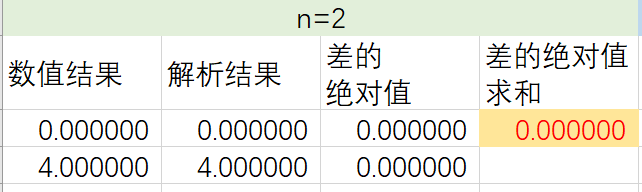
\includegraphics[width=0.6\textwidth]{q1-n=2-解析数值比对.png}
        \caption{q1-n=2-解析数值比对}\label{fig:q1-n=2-解析数值比对}
    \end{figure}
    \begin{figure}[H]
        \centering
        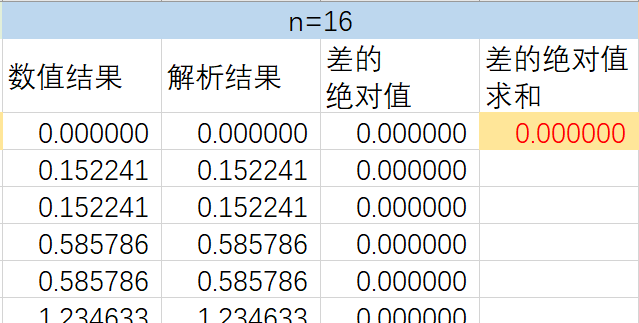
\includegraphics[width=0.6\textwidth]{q1-n=16-解析数值比对.png}
        \caption{q1-n=16-解析数值比对}\label{fig:q1-n=16-解析数值比对}
    \end{figure}
    \begin{figure}[H]
        \centering
        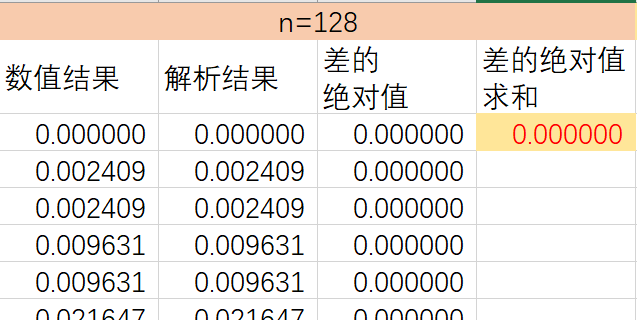
\includegraphics[width=0.6\textwidth]{q1-n=128-解析数值比对.png}
        \caption{q1-n=128-解析数值比对}\label{fig:q1-n=128-解析数值比对}
    \end{figure}
    \begin{figure}[H]
        \centering
        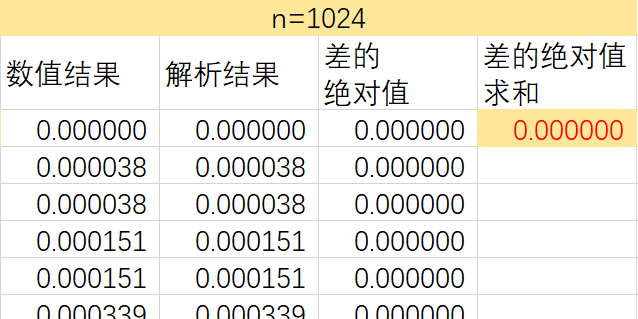
\includegraphics[width=0.6\textwidth]{q1-n=1024-解析数值比对.png}
        \caption{q1-n=1024-解析数值比对}\label{fig:q1-n=1024-解析数值比对}
    \end{figure}

    可以看出,在六位精度下解析结果与数值结果完全相同。

    原始excel表格处理结果见“dataAnalysis.xlsx”中sheet “q1”。

    \subsection{第二问}

    矩阵K变为

    \[
        \begin{pmatrix}
            2+\frac{g_0+g_1\cos 2\pi(\alpha)}{\kappa}&-1& & &-1\\
            -1&2+\frac{g_0+g_1\cos 2\pi(2\alpha)}{\kappa}&-1& &\\
             &-1&\ddots&\ddots& \\
             & &\ddots& &-1\\
            -1& & &-1&2+\frac{g_0+g_1\cos 2\pi(n\alpha)}{\kappa} 
        \end{pmatrix}
        \triangleq K
    \]

    特别地,$g_0=0$时有

    \[
        \begin{pmatrix}
            2+\frac{g_1\cos 2\pi(\alpha)}{\kappa}&-1& & &-1\\
            -1&2+\frac{g_1\cos 2\pi(2\alpha)}{\kappa}&-1& &\\
             &-1&\ddots&\ddots& \\
             & &\ddots& &-1\\
            -1& & &-1&2+\frac{g_1\cos 2\pi(n\alpha)}{\kappa} 
        \end{pmatrix}
        \triangleq K_0
    \]

    且

    \[K=K_0+\frac{g_0}{\kappa}I\]

    那么,如果K,$K_0$的本征值谱为$\lambda,\lambda_0$,那么有$\lambda=\lambda_0+g_0/\kappa$,于是,$c=2-\lambda+g_0/\kappa=2-\lambda_0$。
    因此,为简便起见在之后的小问中,我们都将$g_0$置零,求出$K_0$的本征值谱,再用$c=2-\lambda_0$得到c值。

    本文中,$\alpha=1/2,\gamma=2,n=720$,$K_0$如下

    \[
        \begin{pmatrix}
            0&-1& & & & & & &-1\\
            -1&4&-1& & & & & &\\
             &-1&0&-1& & & & & \\
             & &-1&4& -1& & & &\\
             & & &-1&0&-1& & &\\
             &&&&-1 & \ddots&\ddots& \\
             &&&&& \ddots& && -1\\
            -1& & & & & & &-1&4 
        \end{pmatrix}
    \]

    求解源代码见附件。
    输出结果见"q2-N=720.txt"第一列。

    \subsection{第三问}

    传输矩阵定义如下

    \begin{align*}
        \begin{pmatrix}
            x_3\\
            x_2
        \end{pmatrix}&=
        \begin{pmatrix}
            c+\gamma & -1\\
            1&0
        \end{pmatrix}
        \begin{pmatrix}
            c-\gamma & -1\\
            1&0
        \end{pmatrix}
        \begin{pmatrix}
            x_1\\
            x_0
        \end{pmatrix}\\
        &=
        \begin{pmatrix}
            c^2-\gamma^2-1 & -c-\gamma\\
            c-\gamma&-1
        \end{pmatrix}
        \begin{pmatrix}
            x_1\\
            x_0
        \end{pmatrix}
    \end{align*}

    于是

    \begin{align*}
        \begin{pmatrix}
            x_1\\
            x_0
        \end{pmatrix}
        =
        \begin{pmatrix}
            x_{n+1}\\
            x_n
        \end{pmatrix}
        =
        \begin{pmatrix}
            c^2-\gamma^2-1 & -c-\gamma\\
            c-\gamma&-1
        \end{pmatrix}^{n/2}
        \begin{pmatrix}
            x_1\\
            x_0
        \end{pmatrix}
    \end{align*}

    这里需要n为偶数。

    记传输矩阵的特征值$\eta_\pm $

    要使上式成立,必有$\eta_\pm=exp[\pm i 4\pi k/n]$
    于是有$\eta_++\eta_-=2\cos\frac{4\pi k}{n}$。
    而根据传输矩阵$\eta_++\eta_-=c^2-\gamma^2-2$,联立得到

    \begin{align}
        c^2=\gamma^2+2(1+\cos\frac{4\pi k}{n})
    \end{align}

    由上式可到,$c^2\in[\gamma^2,{\gamma^2+4}]$,则
    $c\in [-\sqrt{\gamma^2+4},-\gamma]\bigcup[\gamma,\sqrt{\gamma^2+4}]$

    $\gamma>0$,于是c分布在两个区间。

    可在第二问的代码中增加一些输出,比对解析和数值结果。

    同时输出特征值的平方,并输出$\gamma^2+2(1+\cos\frac{4\pi k}{n},k=1,2,\cdots,n$,输出结果见"q2-N=720.txt"第二、三列。

    将结果复制到excel中,类似第一问的方法,列内排序、两列作差取绝对值、差的绝对值求和。
    得到

    \begin{figure}[H]
        \centering
        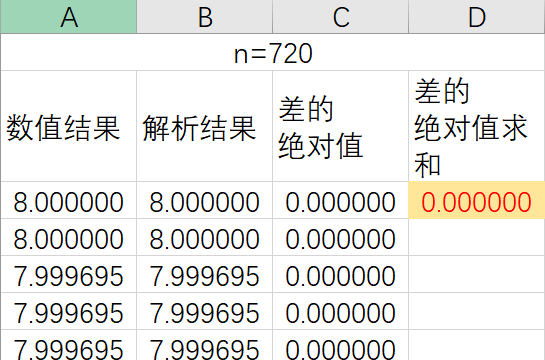
\includegraphics[width=0.6\textwidth]{q3解析数值比对.png}
        \caption{q3解析数值比对}\label{fig:q3解析数值比对}
    \end{figure}

    可见,解析结果与数值结果在六位小数精度下完全吻合。

    原始excel表格处理结果见“dataAnalysis.xlsx”中sheet “q2”。
    \subsection{第四问}

    $\alpha=1/3$时

    \[
        K_0=\begin{pmatrix}
            2&-1& & & & & & &-1\\
            -1&2&-1& & & & & &\\
             &-1&4&-1& & & & & \\
             & &-1&2& -1& & & &\\
             & & &-1&2&-1& & &\\
             &&&&-1 & \ddots&\ddots& \\
             &&&&& \ddots& && -1\\
            -1& & & & & & &-1&4 
        \end{pmatrix}
    \]

    这里要求n是3的倍数。

    $\alpha=1/4$时

    \[
        K_0=\begin{pmatrix}
            2&-1& & & & & & &-1\\
            -1&0&-1& & & & & &\\
             &-1&2&-1& & & & & \\
             & &-1&4& -1& & & &\\
             & & &-1&2&-1& & &\\
             &&&&-1 & \ddots&\ddots& \\
             &&&&& \ddots& && -1\\
            -1& & & & & & &-1&4 
        \end{pmatrix}
    \]

    这里要求n是4的倍数。

    本问编写了一个只需调制$\alpha,N,r$就可以给出本征值组的程序,具体见附录。

    我们不妨还取n=720,$\gamma=2$,数值计算的结果见"q4-a=0.33.txt""q4-a=0.25.txt"。

    将得到的数据降序排列画出如下图像

    \begin{figure}[H]
        \centering
        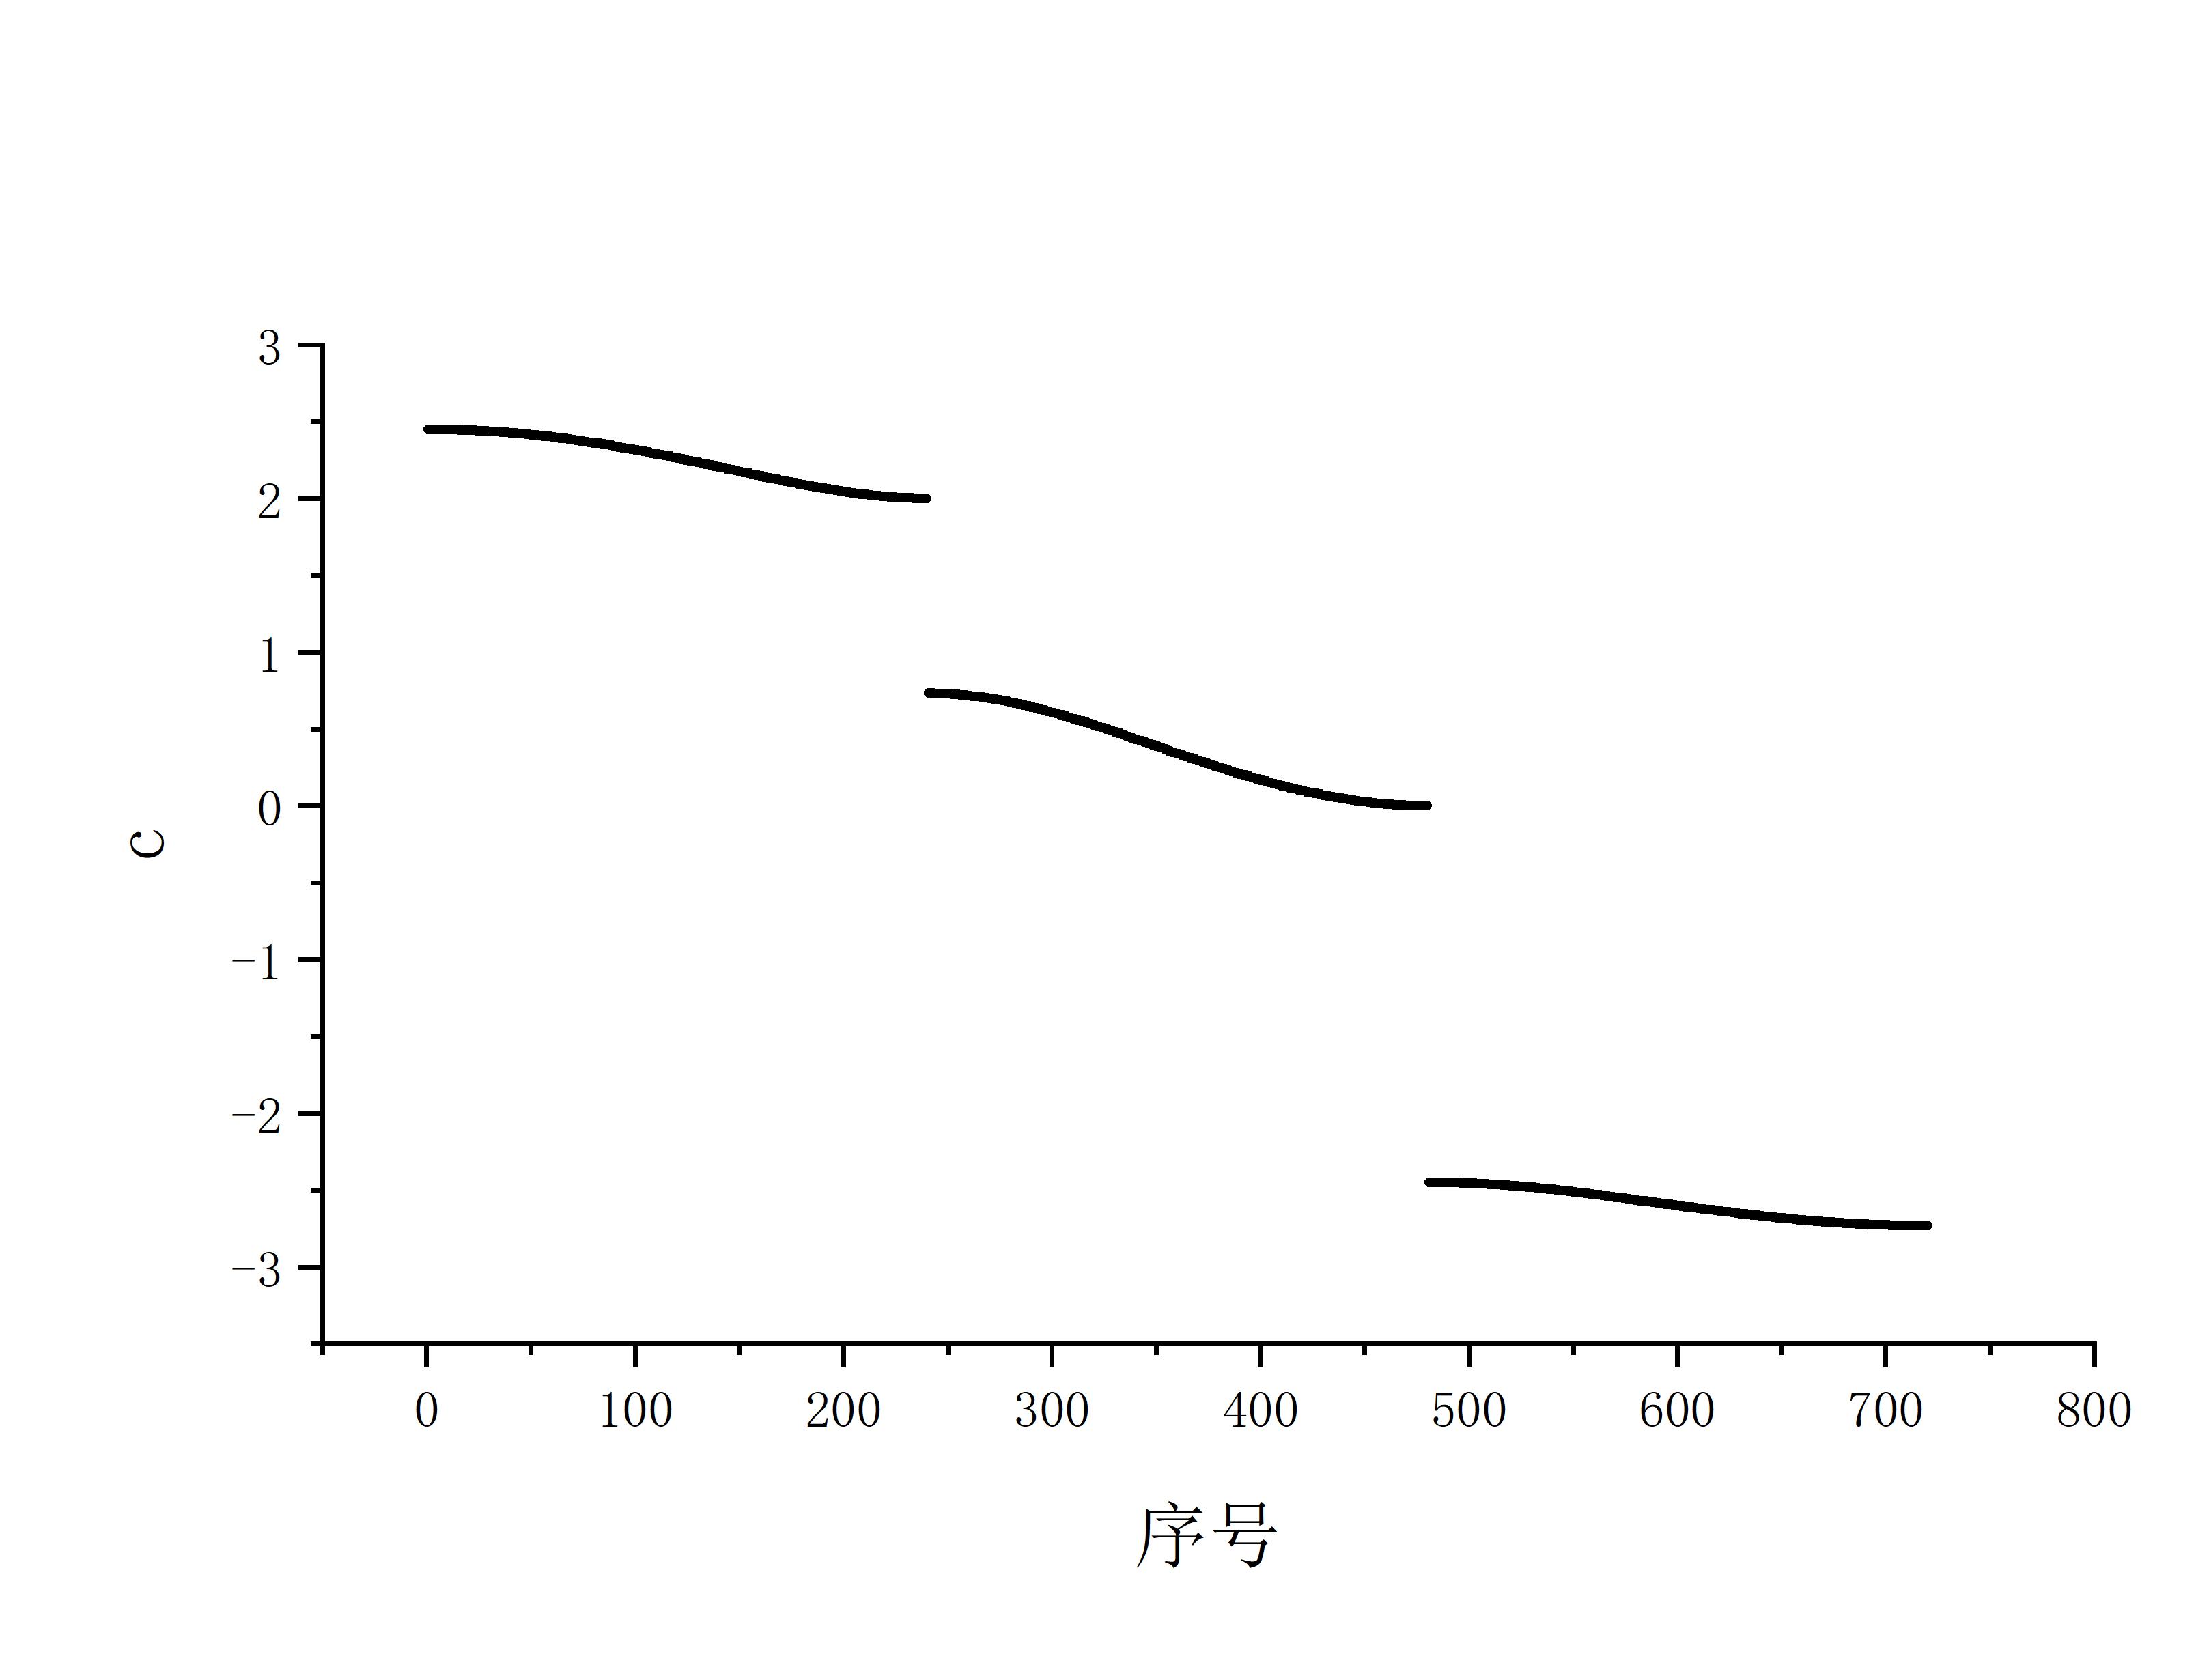
\includegraphics[width=0.6\textwidth]{q4-a=0.33特征值分布图.jpg}
        \caption{q4-a=0.33特征值分布图}\label{fig:q4-a=0.33特征值分布图}
    \end{figure}

    \begin{figure}[H]
        \centering
        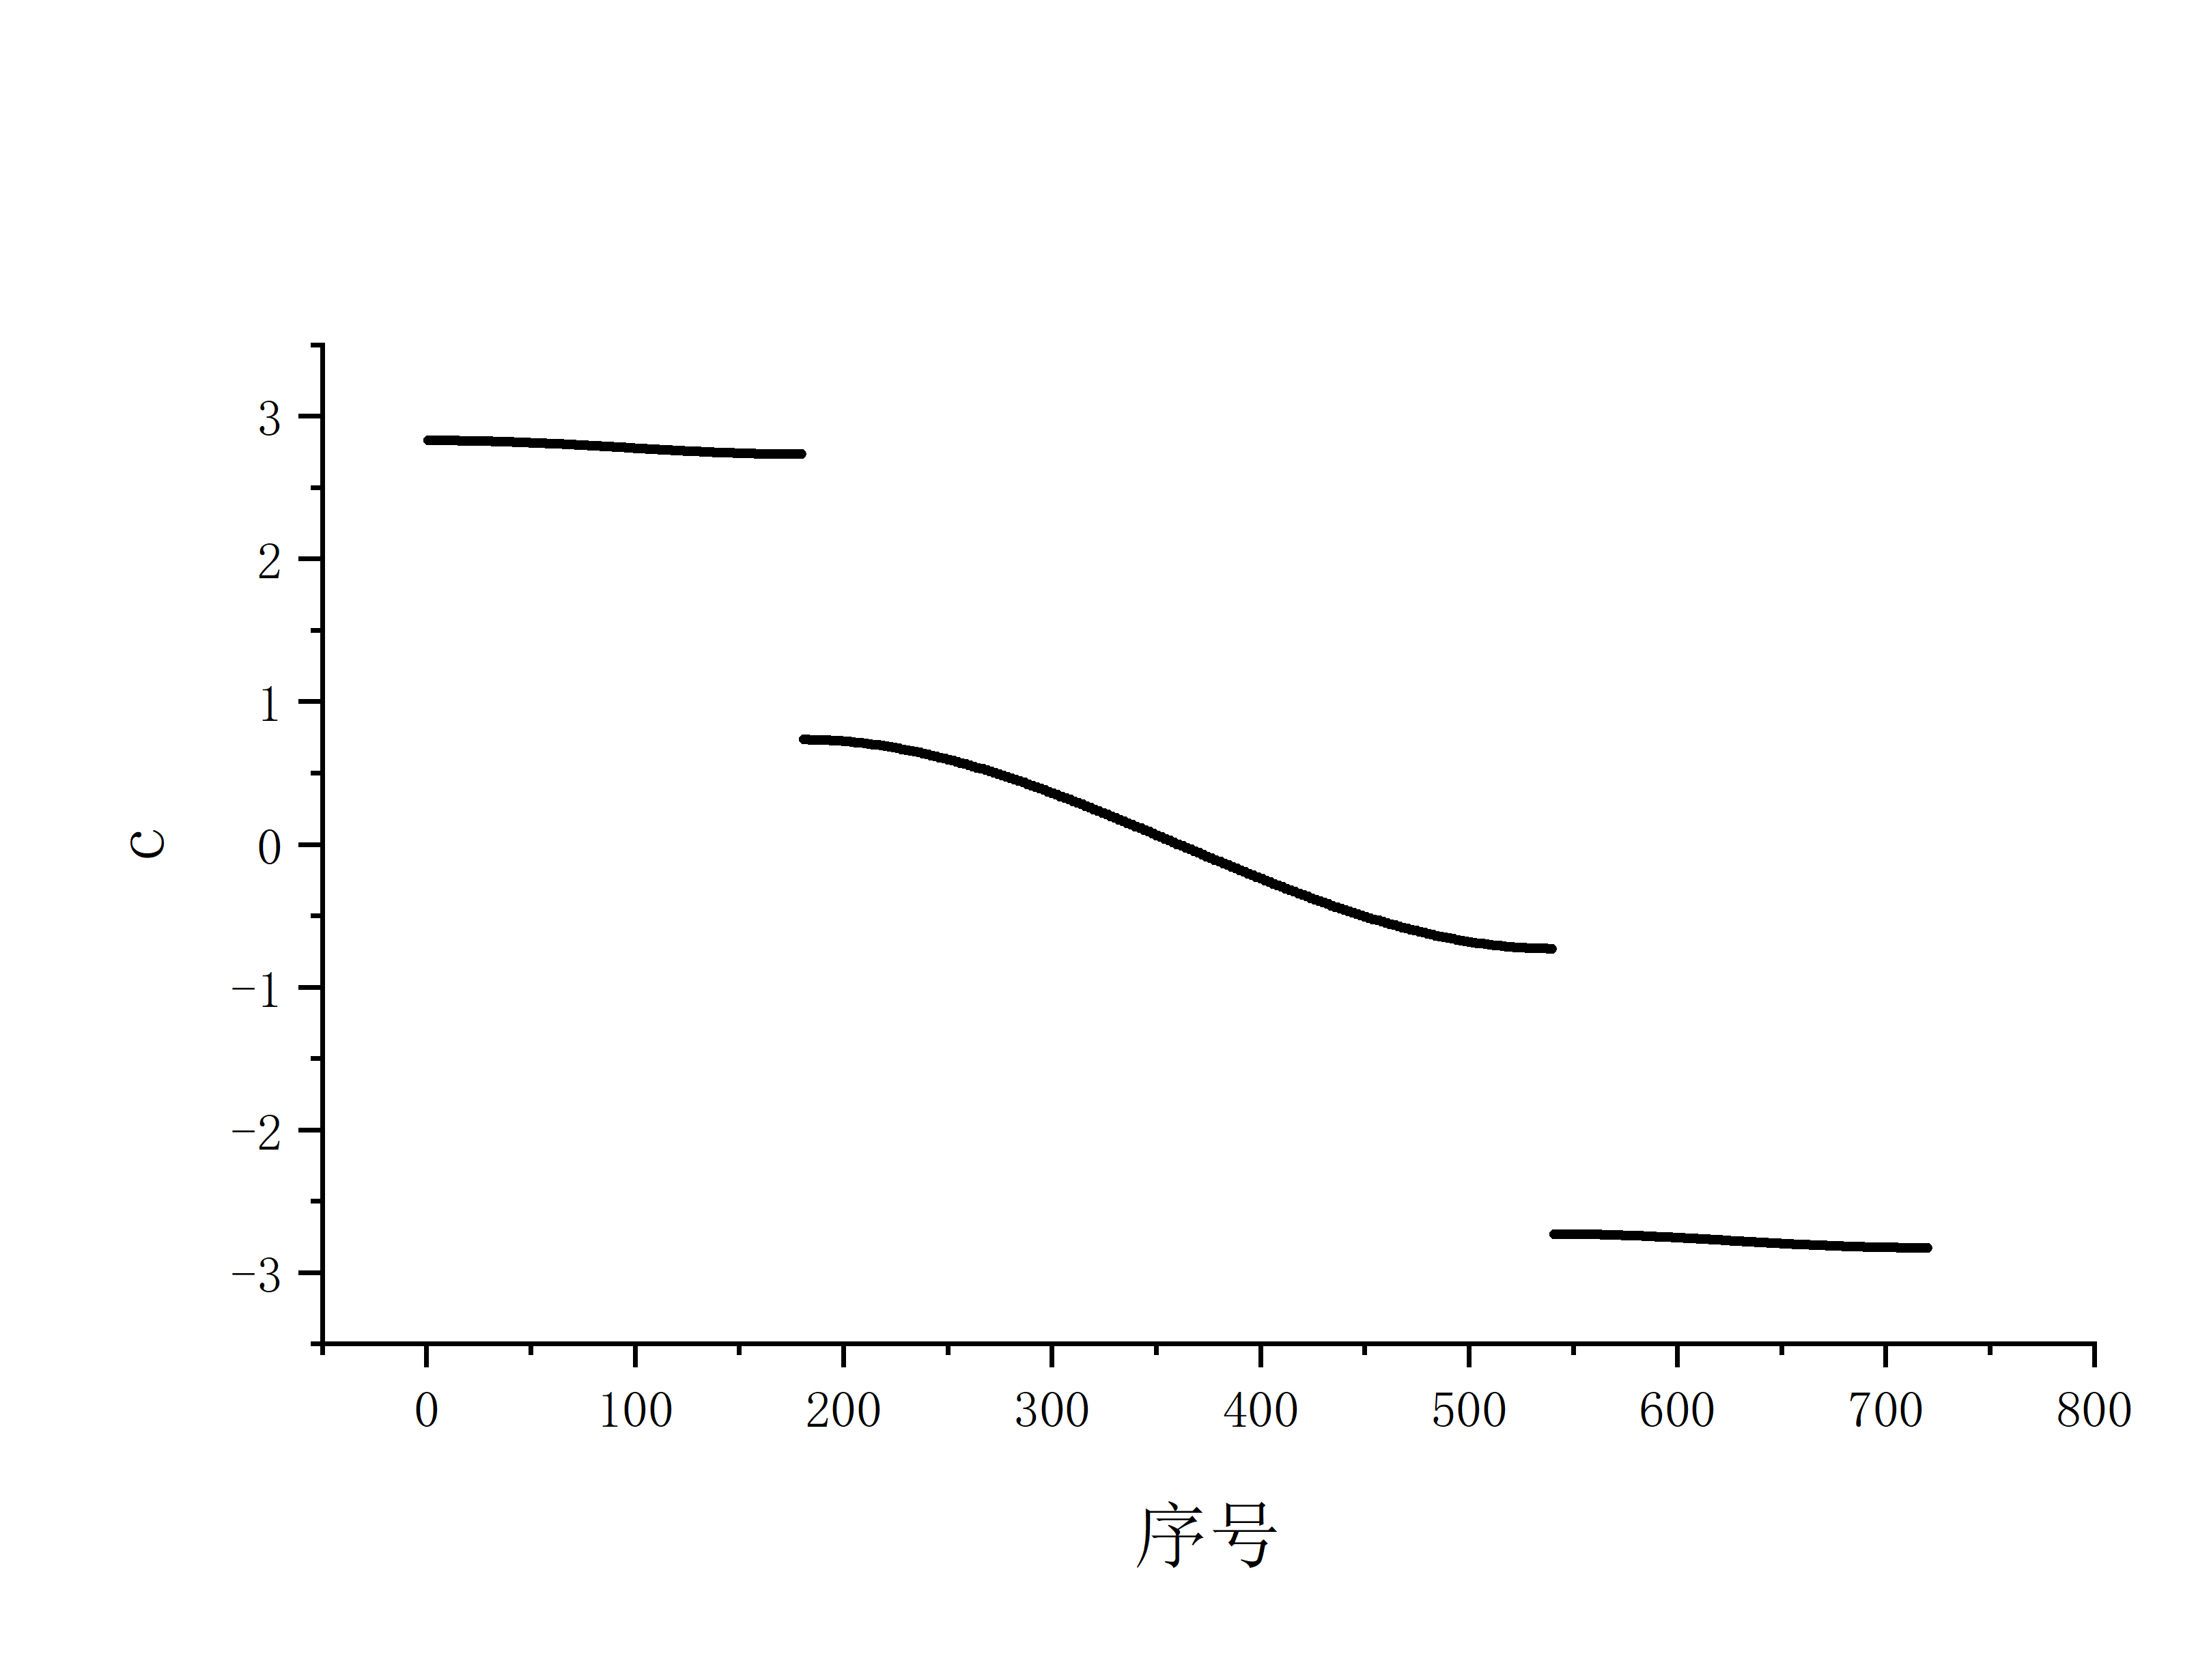
\includegraphics[width=0.6\textwidth]{q4-a=0.25特征值分布图.jpg}
        \caption{q4-a=0.25特征值分布图}\label{fig:q4-a=0.25特征值分布图}
    \end{figure}

    可以数值地给出

    \begin{align}
        \alpha&=1/3, c\in[-2.732051,-2.449490]\bigcup[0,0.732051]\bigcup[2,2.449490]\\
        \alpha&=1/4, c\in[-2.828427,-2.732051]\bigcup[-0.732051,0,732051]\bigcup[2.732051,2.828427]
    \end{align}\label{ali:q4数值}

    类似的,可以解析的给出c地取值范围

    传输矩阵为

    \begin{align*}
        \alpha&=1/3:\\
        &\begin{pmatrix} 
            c+\gamma & -1\\
            1&0
        \end{pmatrix}
        \begin{pmatrix} 
            c-\frac{1}{2}\gamma & -1\\
            1&0
        \end{pmatrix}
        \begin{pmatrix}
            c-\frac{1}{2}\gamma & -1\\
            1&0
        \end{pmatrix}\\
        &=
        \begin{pmatrix}
            \frac{1}{4}(-8c+4c^3-2\gamma-3c\gamma^2+\gamma^3) & 1-(c-\gamma/2)(c+\gamma)\\
            -1+(c-\gamma/2)^2&\frac{1}{2}(-2c+\gamma)
        \end{pmatrix}\\
        \alpha&=1/4:\\
        &\begin{pmatrix} 
            c+\gamma & -1\\
            1&0
        \end{pmatrix}
        \begin{pmatrix} 
            c & -1\\
            1&0
        \end{pmatrix}
        \begin{pmatrix} 
            c-\gamma & -1\\
            1&0
        \end{pmatrix}
        \begin{pmatrix}
            c & -1\\
            1&0
        \end{pmatrix}\\
        &=\begin{pmatrix}
            1+c^4-cr-c^2(3+r^2) & c(2-c^2+r^2)\\
            c(-2+c^2-cr)&1-c^2+cr
        \end{pmatrix}
    \end{align*}

    类似第三问的推导过程,传输矩阵的特征值$\eta_\pm=\exp[\pm i 2\pi \alpha]$,再根据矩阵的性质,特征值之和为对角元之和,得到

    $\alpha=1/3$时,

    \[c^3+\frac{\gamma ^3}{4}-\frac{3}{4} (\gamma ^2+4) c=2\cos\frac{6\pi k}{n}\]

    $\gamma=2$时,

    \[c^3-6c+2(1-\cos\frac{6\pi k}{n})=0\]

    于是c应取$c^3-6c+h=0,0\leq h\leq 4$时的解。

    \begin{figure}[H]
        \centering
        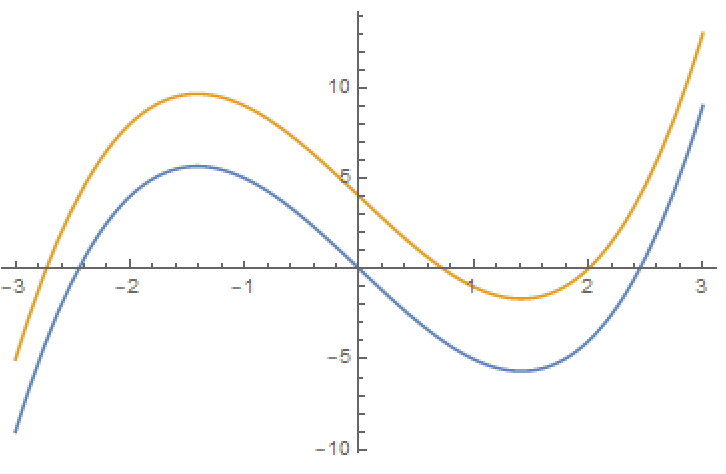
\includegraphics[width=0.3\textwidth]{q4-a=0.33解析计算示意图.png}
    \end{figure}

    画出示意图,h从0变到4的时候,函数从蓝线上升到黄线。函数擦过的x轴就是c可以取到的值。

    于是解方程$c^3-6c=0$得到
    \[c_1=-\sqrt{6},c2=0,c_3=\sqrt{6}\]
    
    解方程$c^3-6c+4=0$得到
    \[c_1=2,c2=-1-\sqrt{3},c_3=-1+\sqrt{3}\]

    得到$c\in[-1-\sqrt{3},-\sqrt{6}]\bigcup[0,-1+\sqrt{3}]\bigcup[2,\sqrt{6}]$

    $\alpha=1/4$时,

    \[c^4-c^2(4+\gamma^2)+2(1-\cos\frac{8\pi k}{n})=0\]

    于是

    \[c^2_\pm=\frac{4+\gamma^2\pm\sqrt{(4+\gamma^2)^2-8(1-\cos\frac{8\pi k}{n})}}{2}\]

    即

    \[c^2\in[0,\frac{4+\gamma^2-\sqrt{(4+\gamma^2)^2-16}}{2}]\bigcup[\frac{4+\gamma^2+\sqrt{(4+\gamma^2)^2-16}}{2},4+\gamma^2]\]

    于是

    \begin{align*}
        c&\in[-c_1,-c_2]\bigcup[-c_3,c_3]\bigcup[c_2,c_1]\\
        c_1&=\sqrt{4+\gamma^2}\\
        c_2&=\sqrt{\frac{4+\gamma^2+\sqrt{(4+\gamma^2)^2-16}}{2}}\\
        c_3&=\sqrt{\frac{4+\gamma^2-\sqrt{(4+\gamma^2)^2-16}}{2}}
    \end{align*}


    当$\gamma=2$有

    \[c\in[-2\sqrt{2},-1-\sqrt{3}]\bigcup[1-\sqrt{3},-1+\sqrt{3}]\bigcup[1+\sqrt{3},2\sqrt{2}]\]

    综上

    \begin{align}
        \alpha&=1/3, c\in[-1-\sqrt{3},-\sqrt{6}]\bigcup[0,-1+\sqrt{3}]\bigcup[2,\sqrt{6}]\\
        \alpha&=1/4, c\in[-2\sqrt{2},-1-\sqrt{3}]\bigcup[1-\sqrt{3},-1+\sqrt{3}]\bigcup[1+\sqrt{3},2\sqrt{2}]
    \end{align}\label{ali:q4解析}

    可以验证,式(6)和(8)、(7)和(9)吻合得很好。

    值得特别说明的是,根据第五问的结论,$\alpha=1/4$时特征值区间将劈裂成4份,但这里数值和解析结果都指出,特征值区间劈裂成3份。
    注意到特征值中央区间关于原点对称分布,如果把原点两侧的部分看成两个区间,那么特征值劈裂成了4份。这里猜测,
    第五问的结论是在把关于原点对称的区间看成2个意义上成立的。

    \subsection{第五问}

    利用第四问代码,只需设置参数,即可完成本问计算,取
    \[n=720,\gamma=2,\alpha=1/5,1/6,1/7\]得到数据见"q5-a=0.2.txt""q5-a=0.166.txt""q5-a=0.142.txt".

    将数据降序排序后获得如下特征值分布图

    \begin{figure}[H]
        \centering
        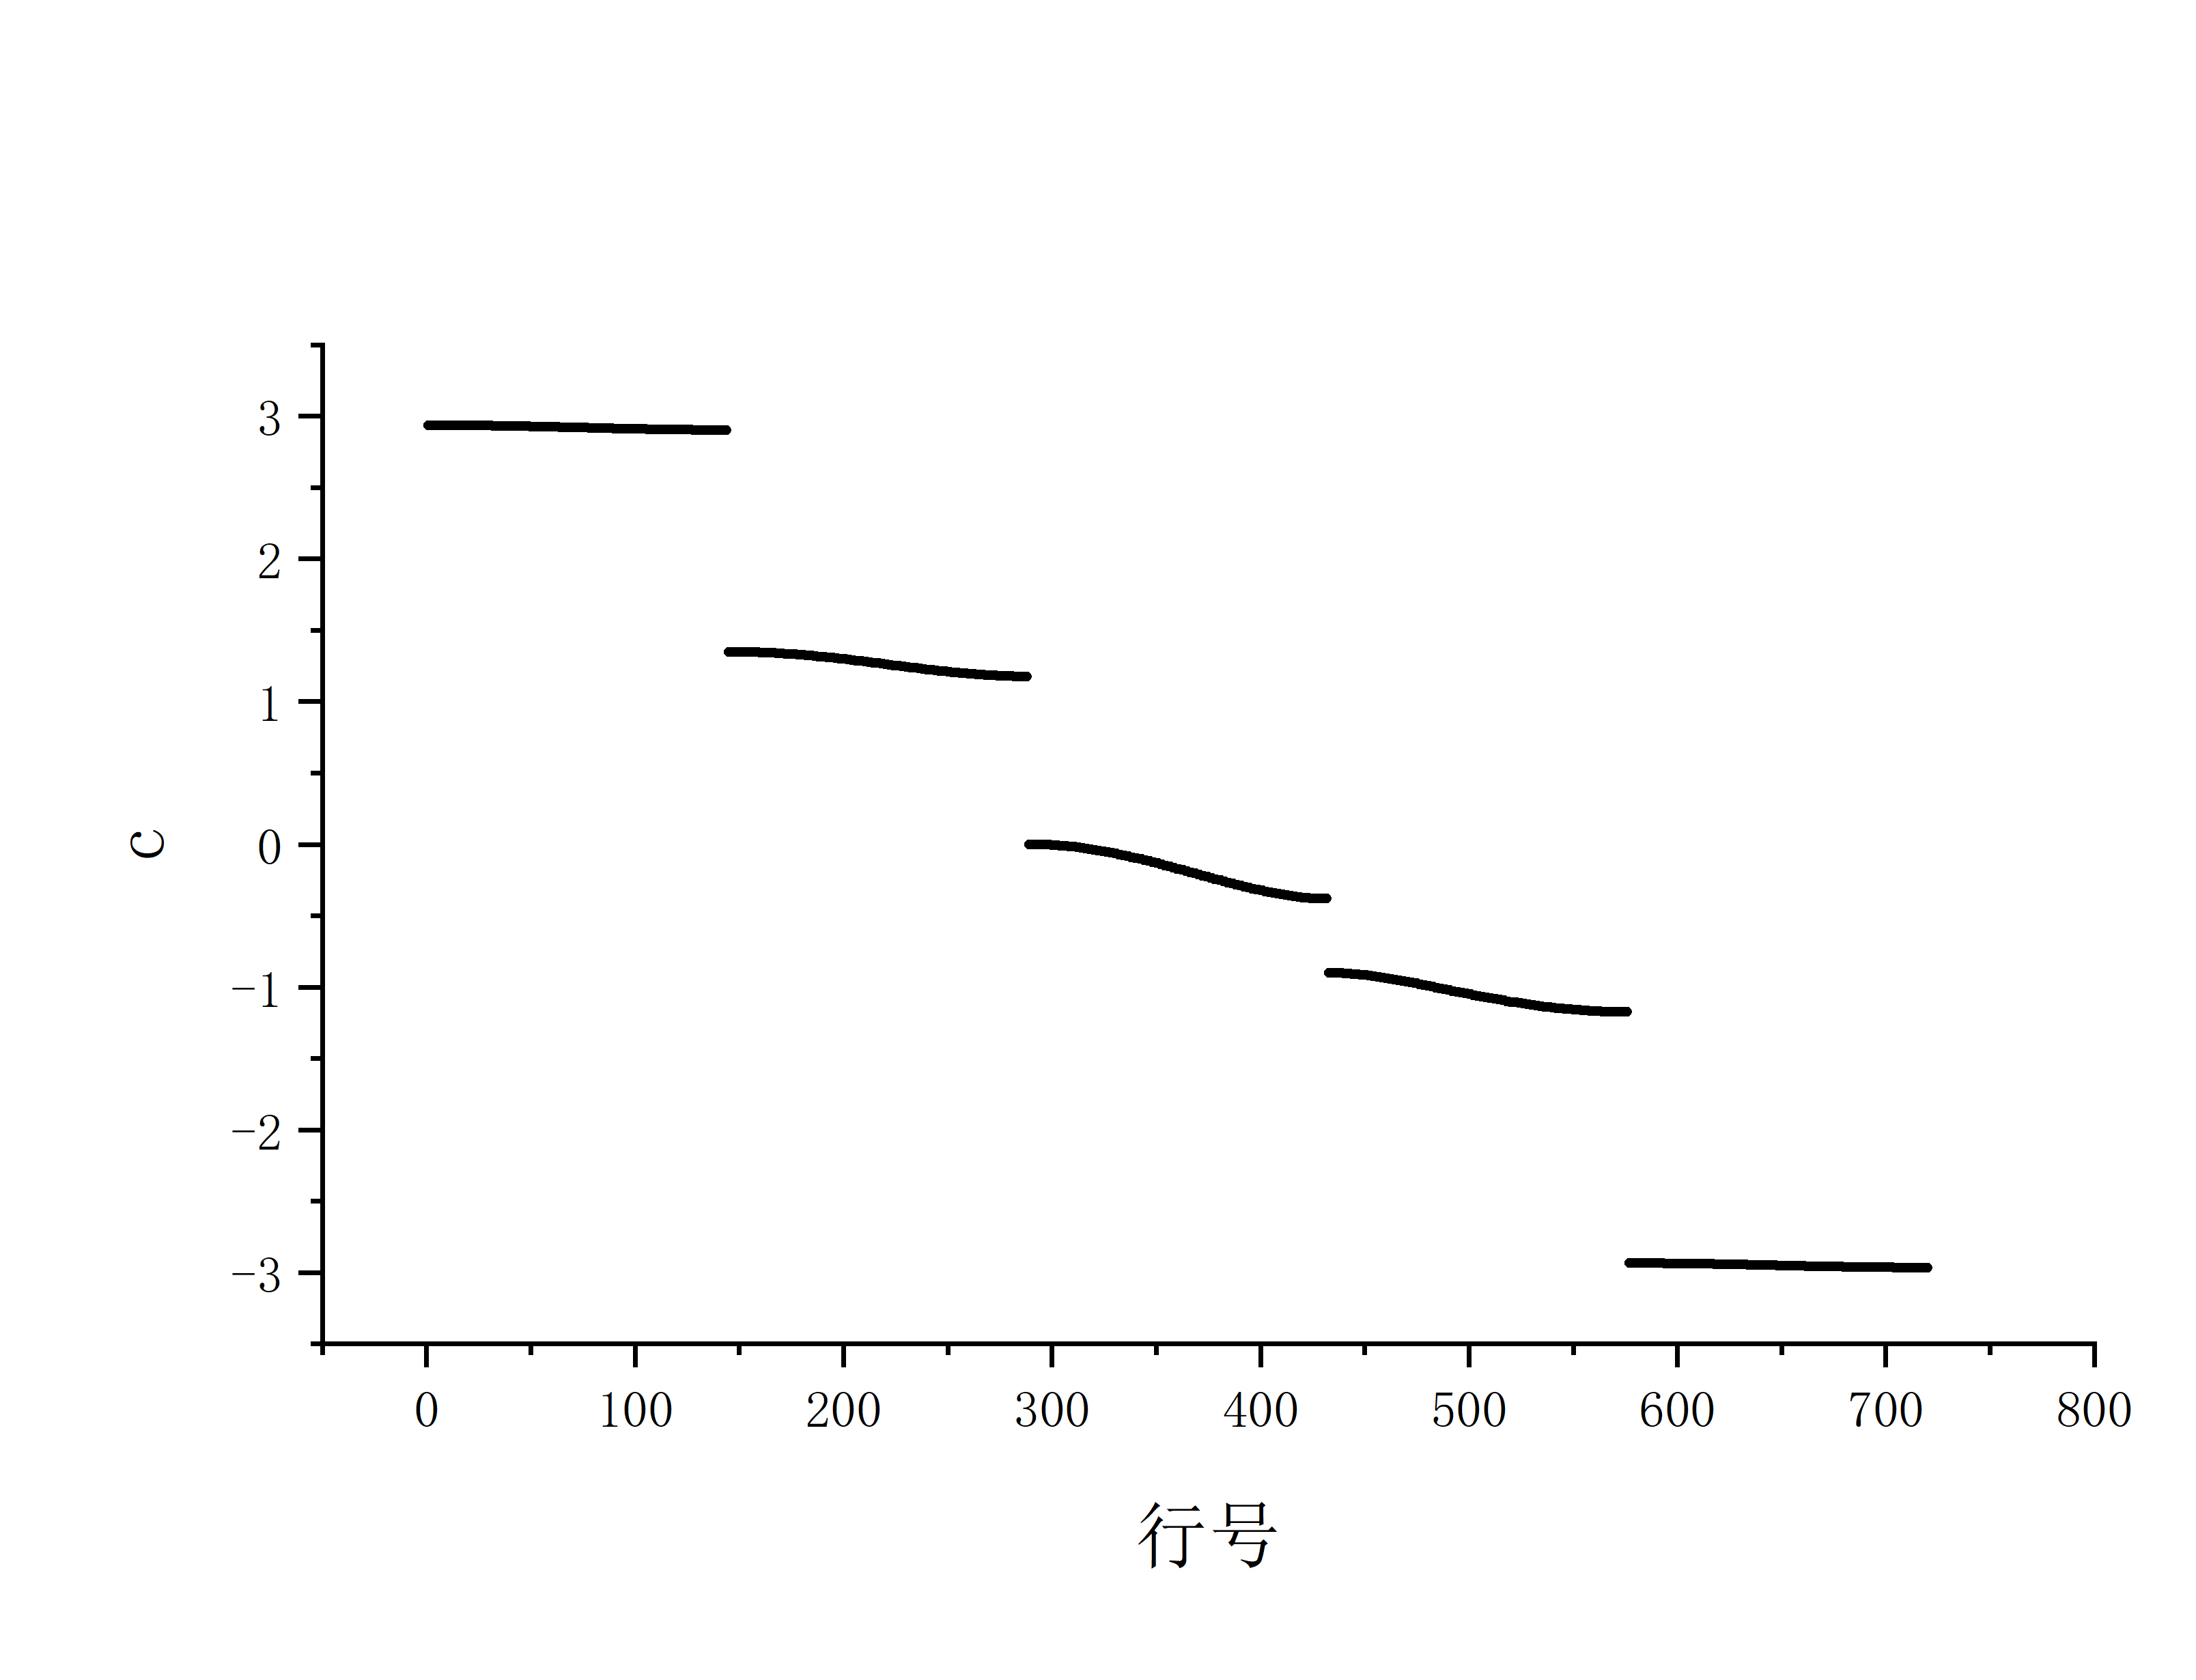
\includegraphics[width=0.6\textwidth]{q5-a=0.2特征值分布图.jpg}
        \caption{q5-a=0.2特征值分布图}\label{fig:q5-a=0.2特征值分布图}
    \end{figure}

    \begin{figure}[H]
        \centering
        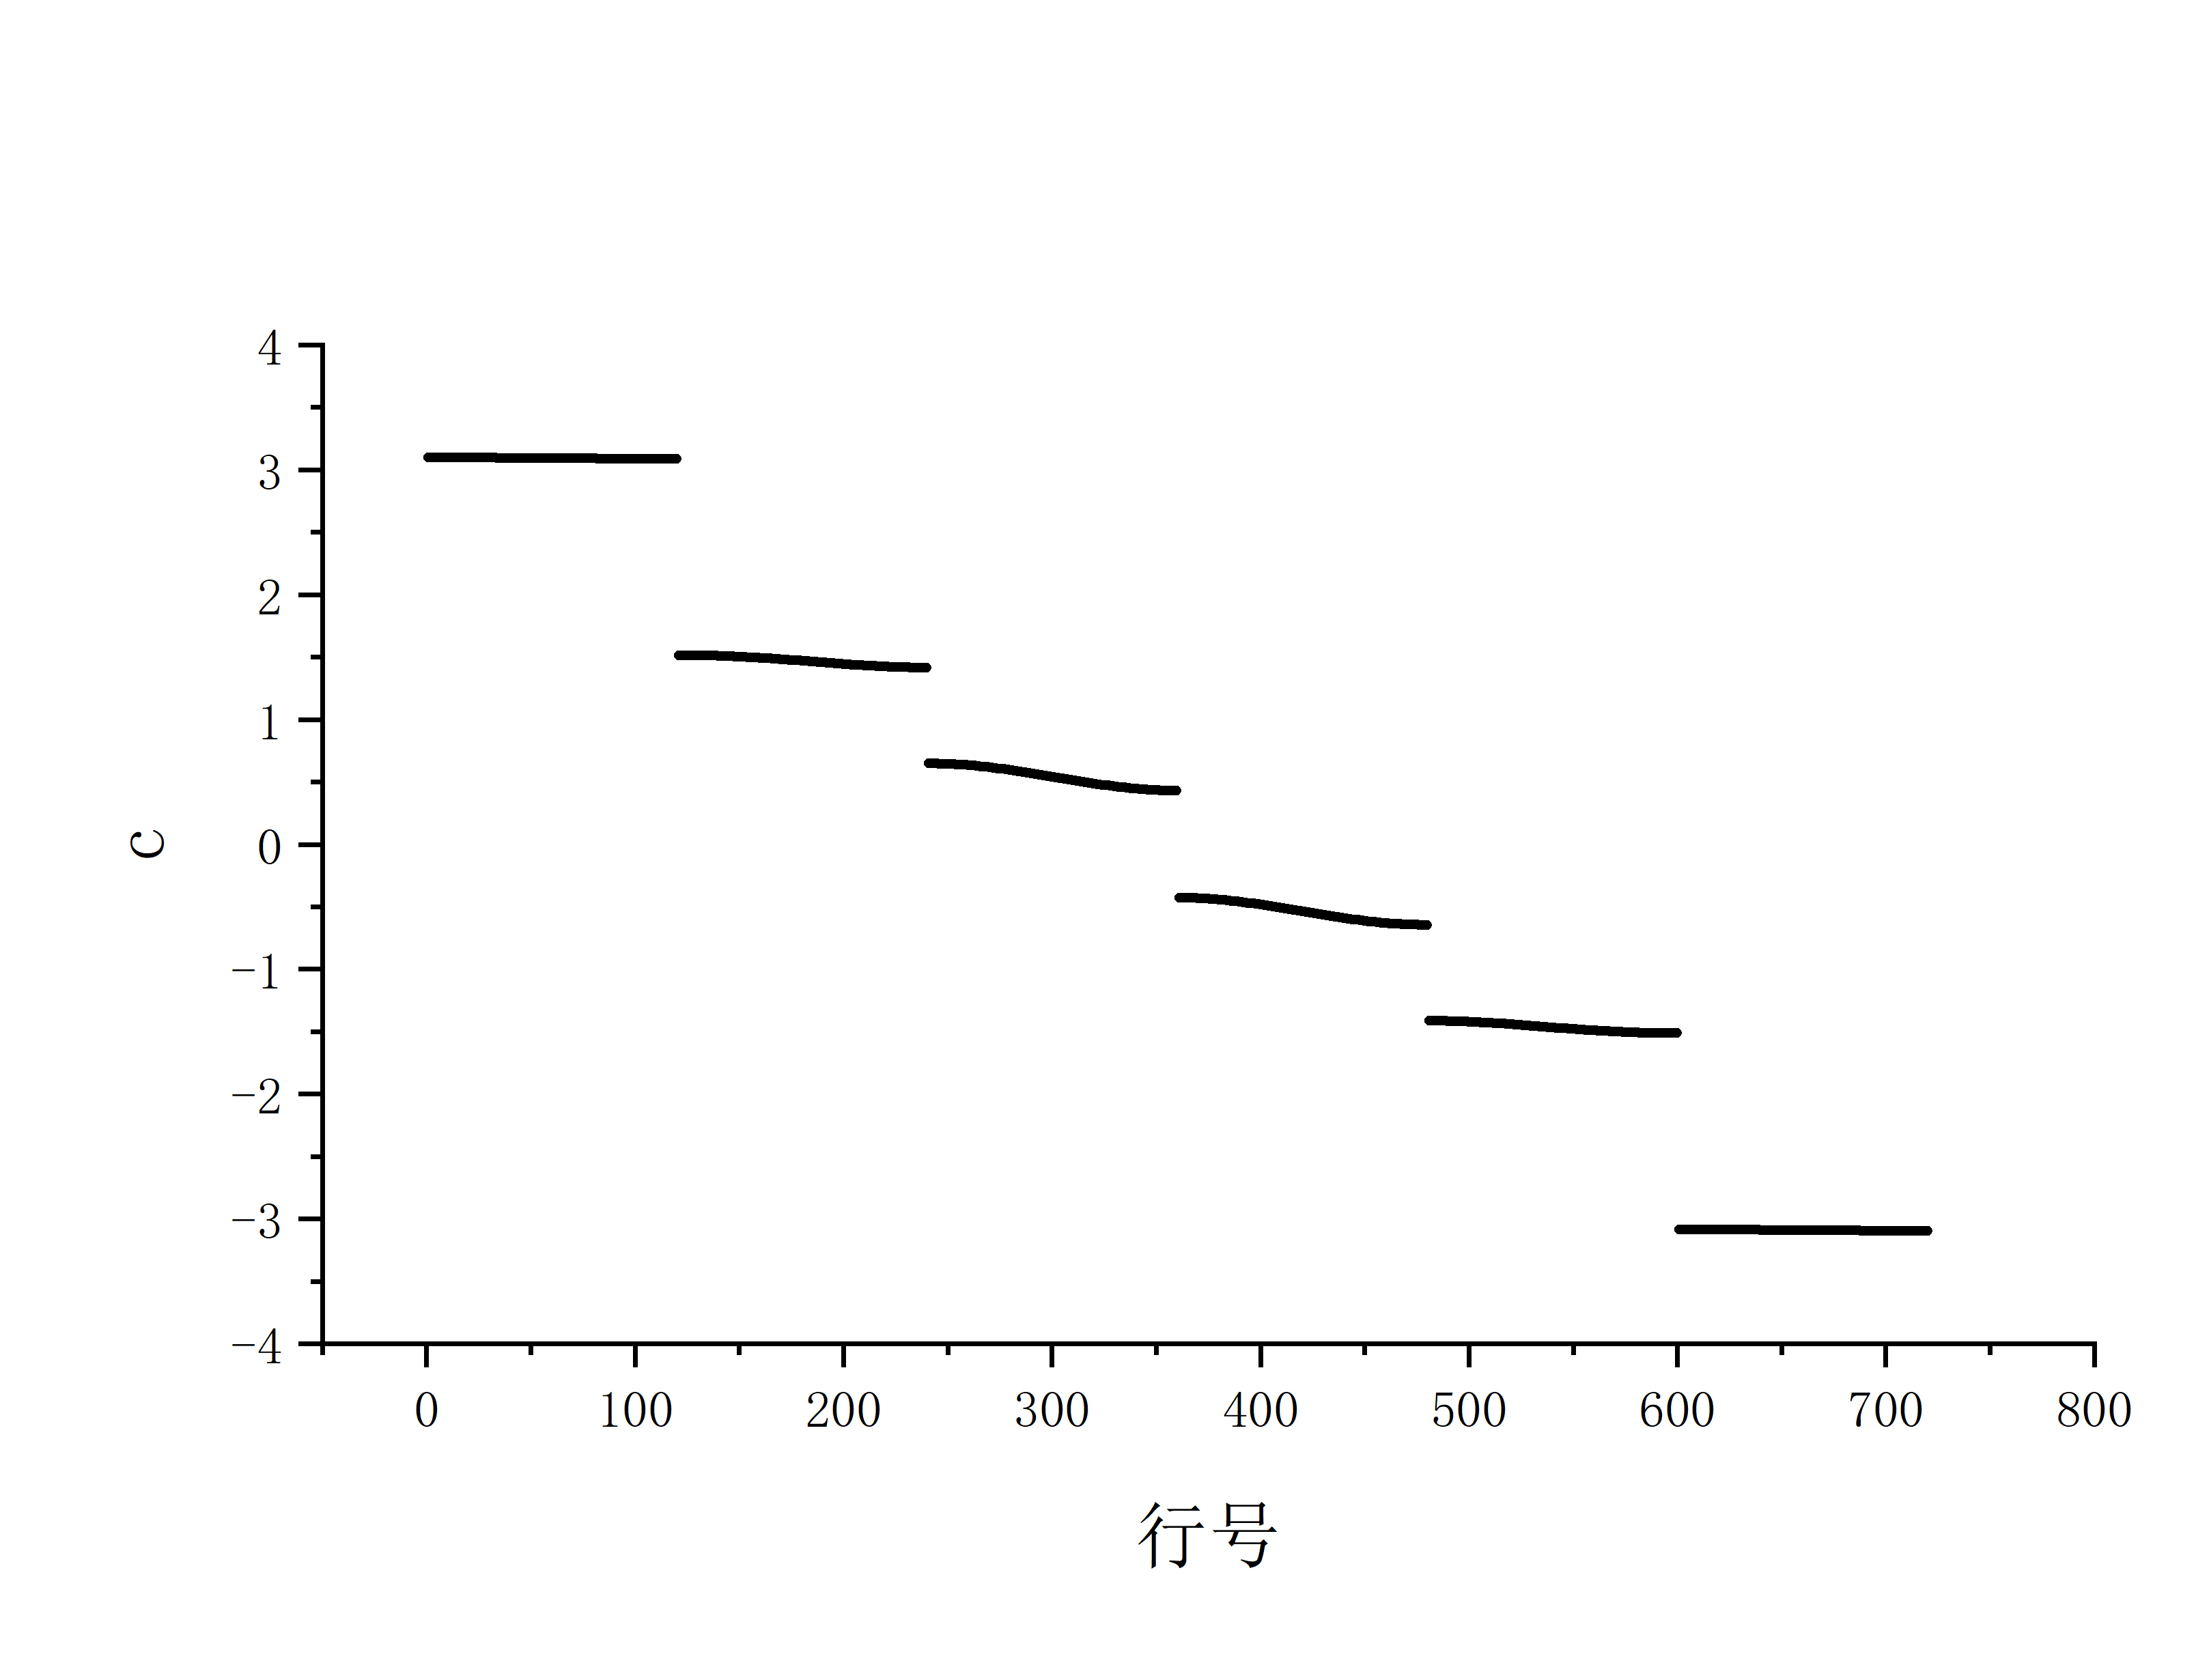
\includegraphics[width=0.6\textwidth]{q5-a=0.166特征值分布图.jpg}
        \caption{q5-a=0.166特征值分布图}\label{fig:q5-a=0.166特征值分布图}
    \end{figure}

    \begin{figure}[H]
        \centering
        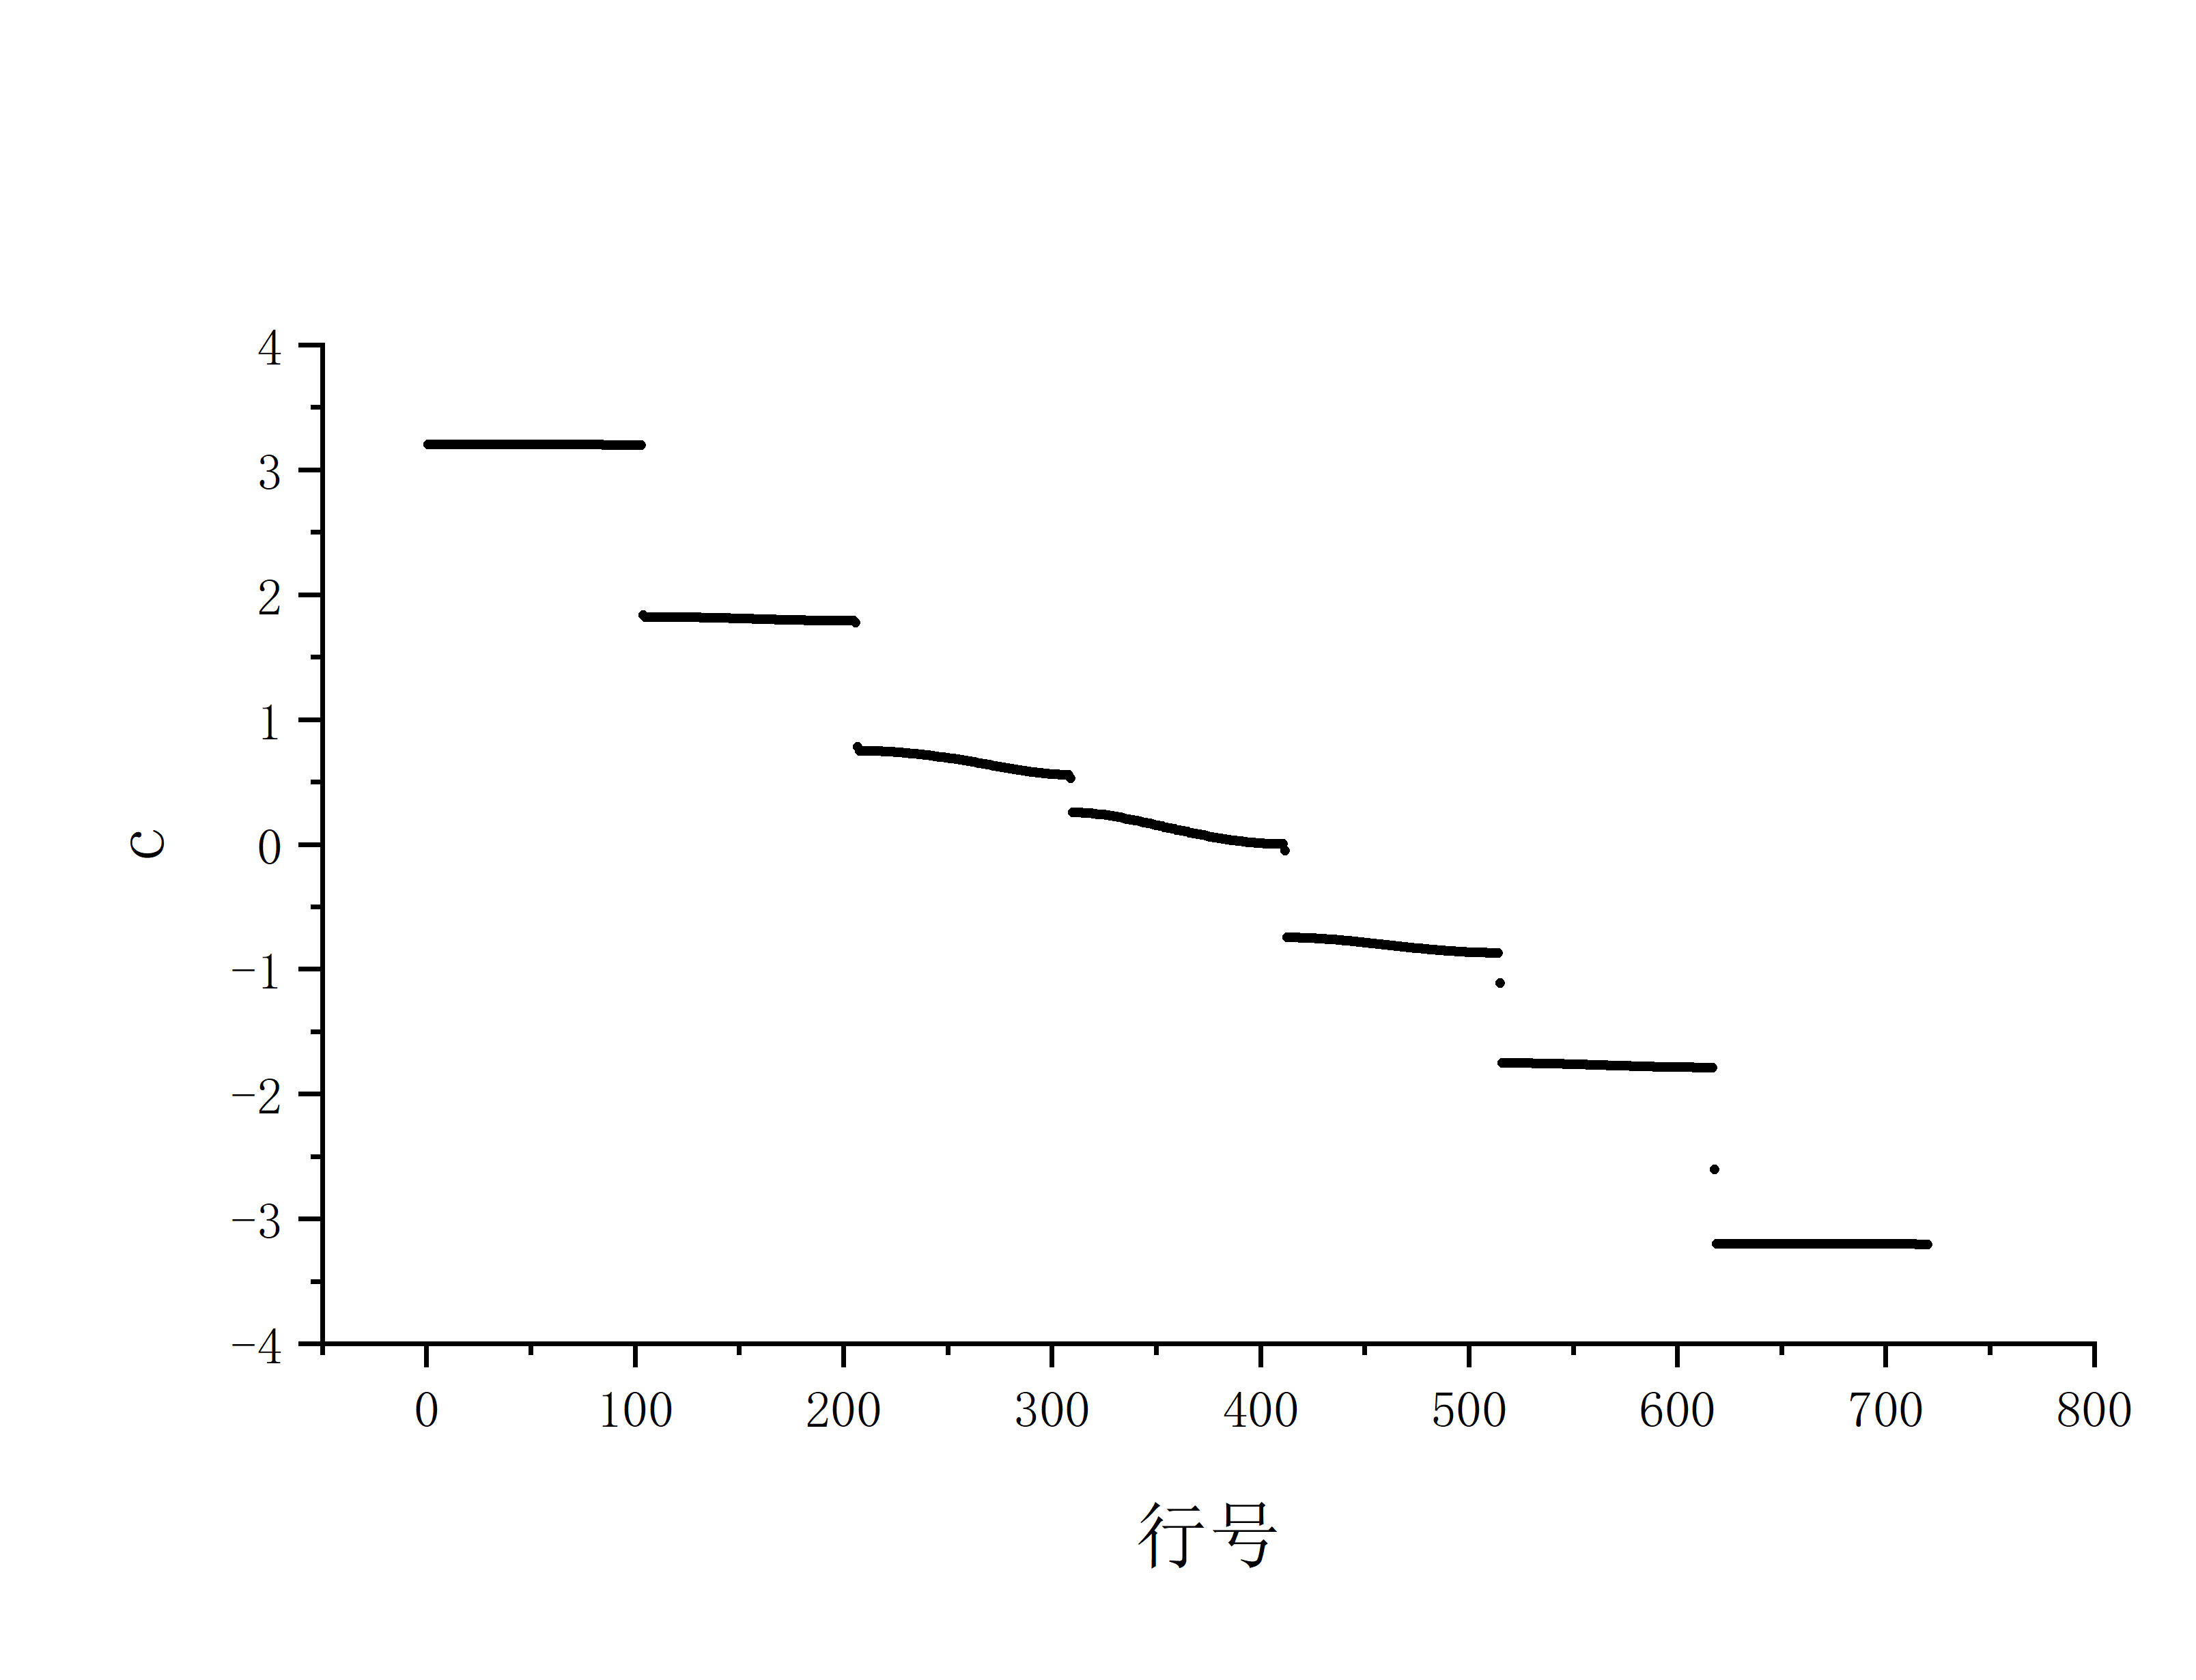
\includegraphics[width=0.6\textwidth]{q5-a=0.142特征值分布图.jpg}
        \caption{q5-a=0.142特征值分布图}\label{fig:q5-a=0.142特征值分布图}
    \end{figure}

    观察到$\alpha=1/5,1/6$时特征值区间都被很好的劈裂成$1/\alpha$份,但$\alpha=1/7$时特征值存在一些孤立散点。猜测可能和n=720不是7的倍数有关。
    改变条件
    \[n=770,\gamma=2,\alpha=1/7\]

    得到数据见"q5-a=0.142-N=770.txt",降序排列绘成下图

    \begin{figure}[H]
        \centering
        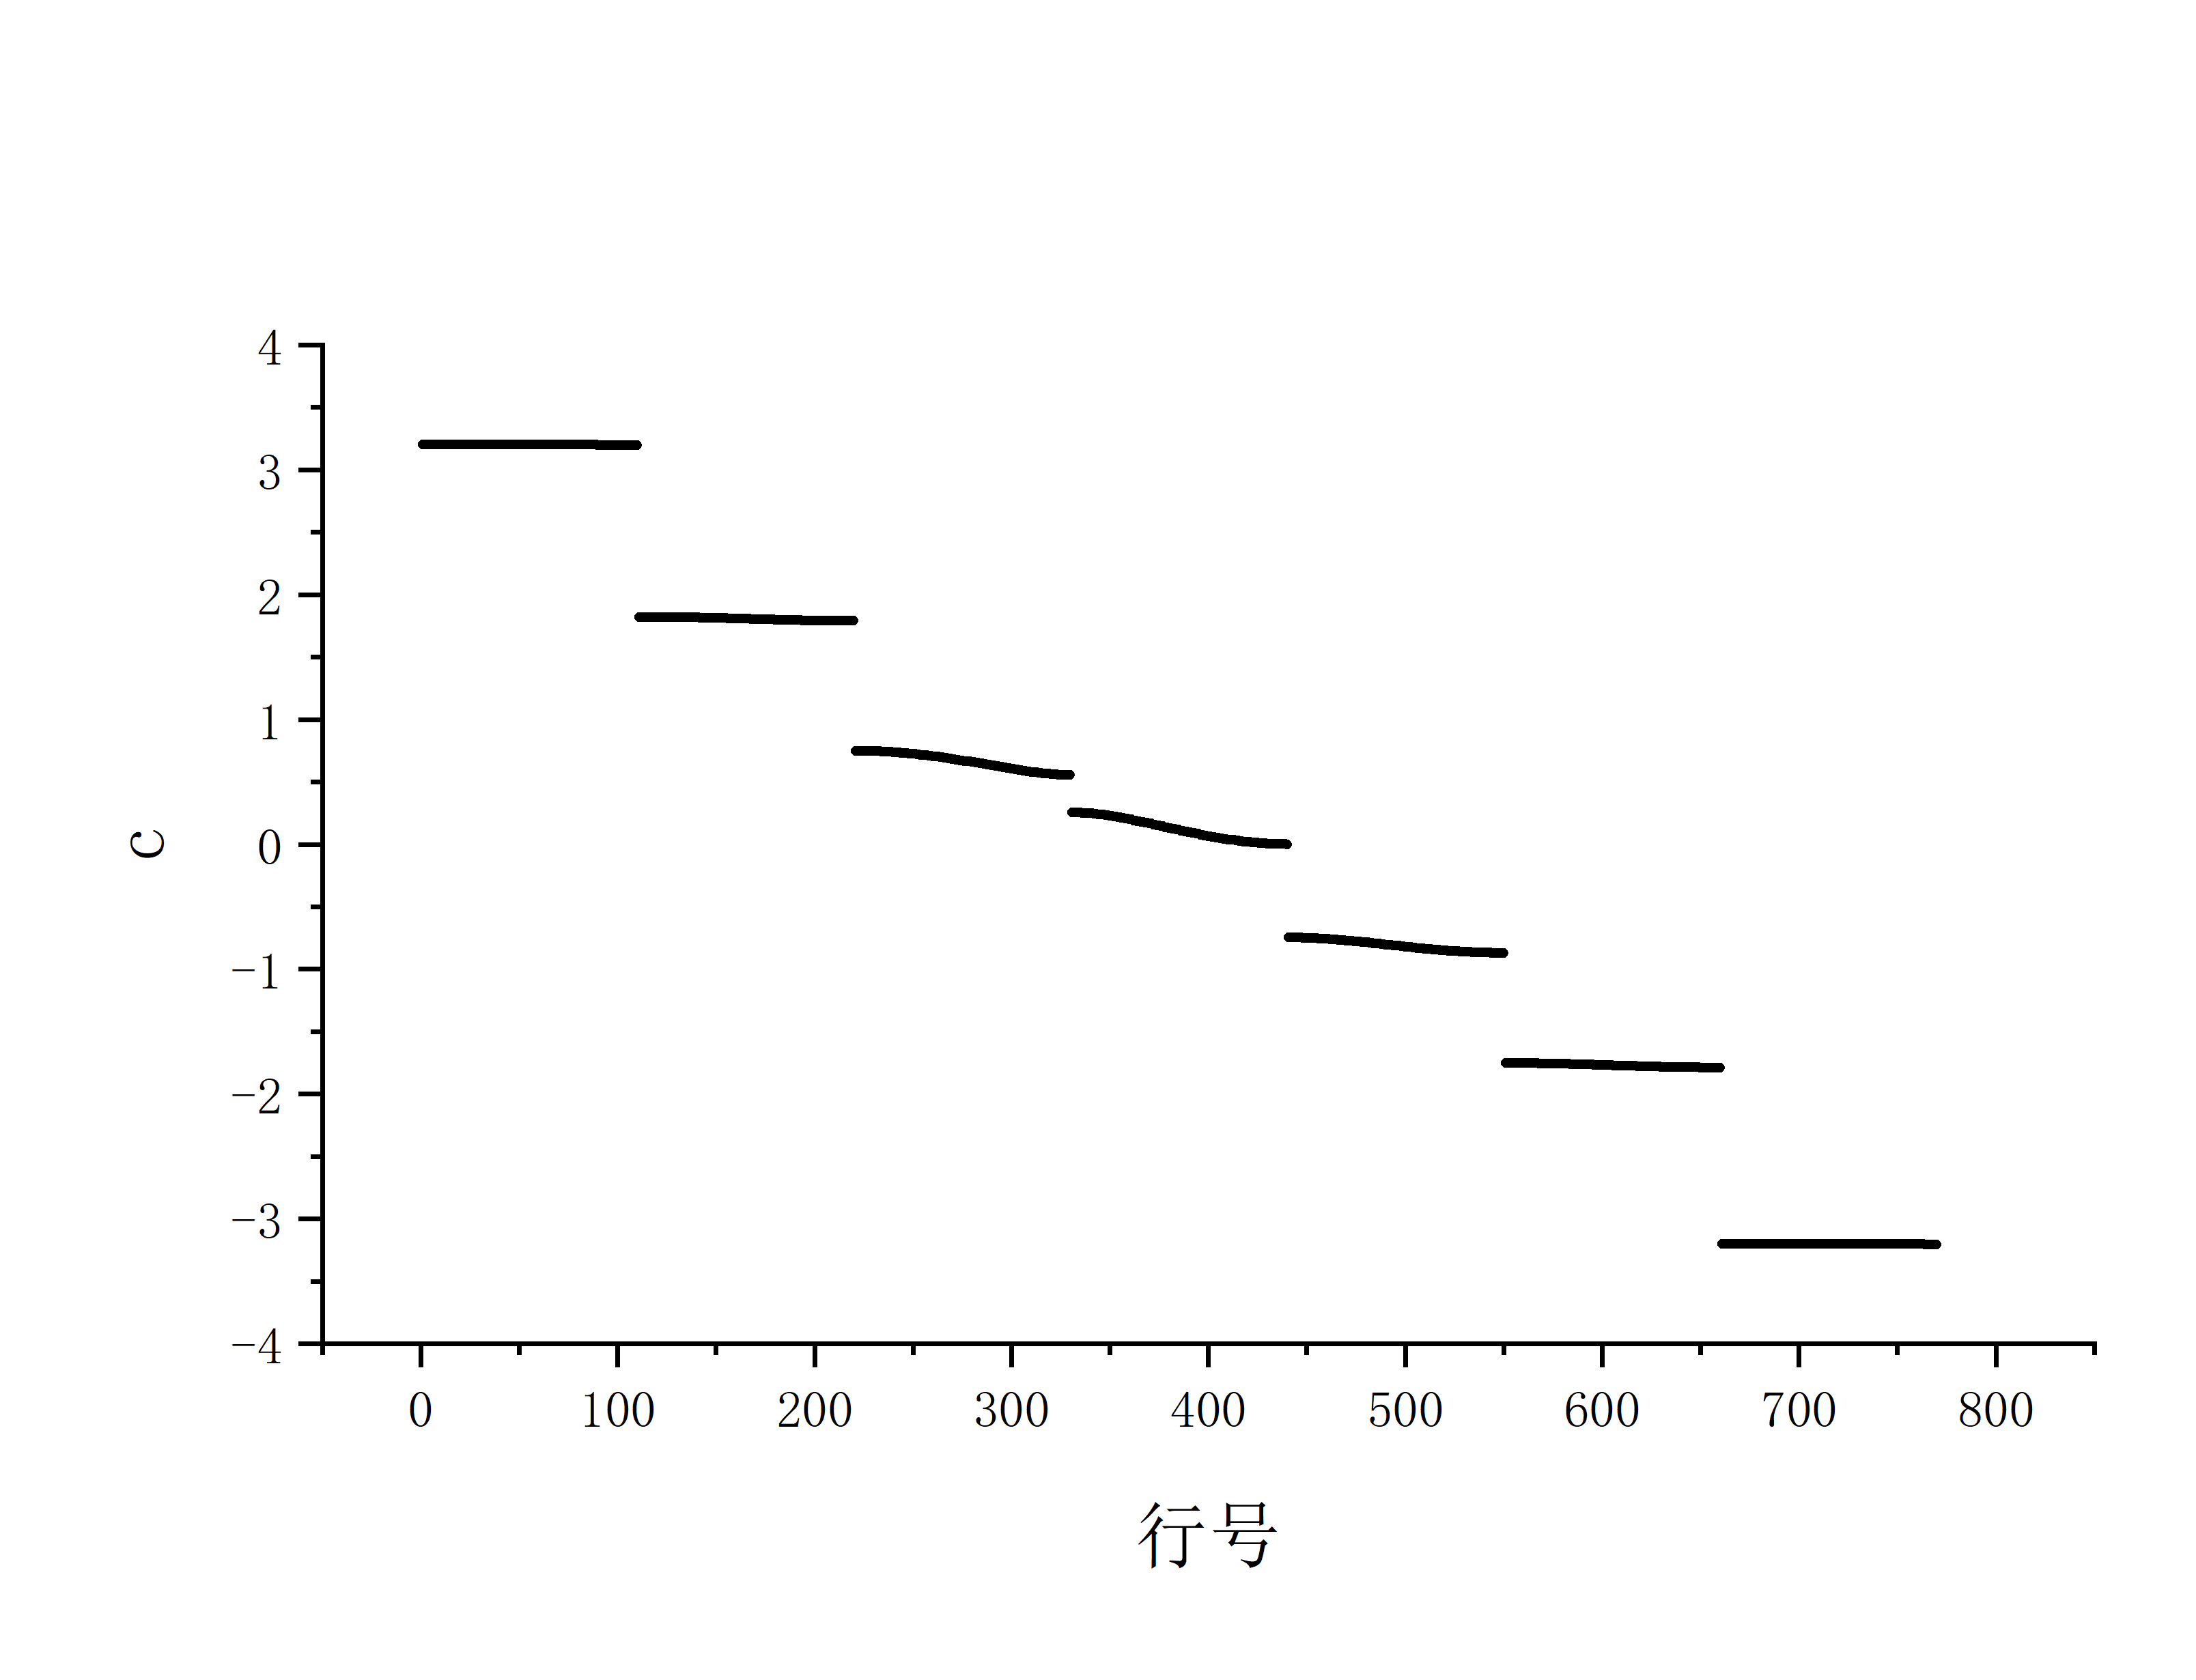
\includegraphics[width=0.6\textwidth]{q5-a=0.142-N=770特征值分布图.jpg}
        \caption{q5-a=0.142-N=770特征值分布图}\label{fig:q5-a=0.142-N=770特征值分布图}
    \end{figure}

    可以看出,散点消失,特征值区间又成了完美的$1/\alpha$份。
    这体现了,想要观察到完美的区间劈裂,n需要是$1/\alpha$的倍数。

    另外,题目中的结论是特征值区间劈裂与$\alpha$分子无关,下面作出验证。

    取

    \[n=770,\gamma=2,\alpha=1/5,2/5,3/5,4/5\]
    
    得到数据见"q5-a=0.2.txt","q5-a=0.4.txt","q5-a=0.6.txt","q5-a=0.8.txt"

    作出$c-\alpha$图,得到

    \begin{figure}[H]
        \centering
        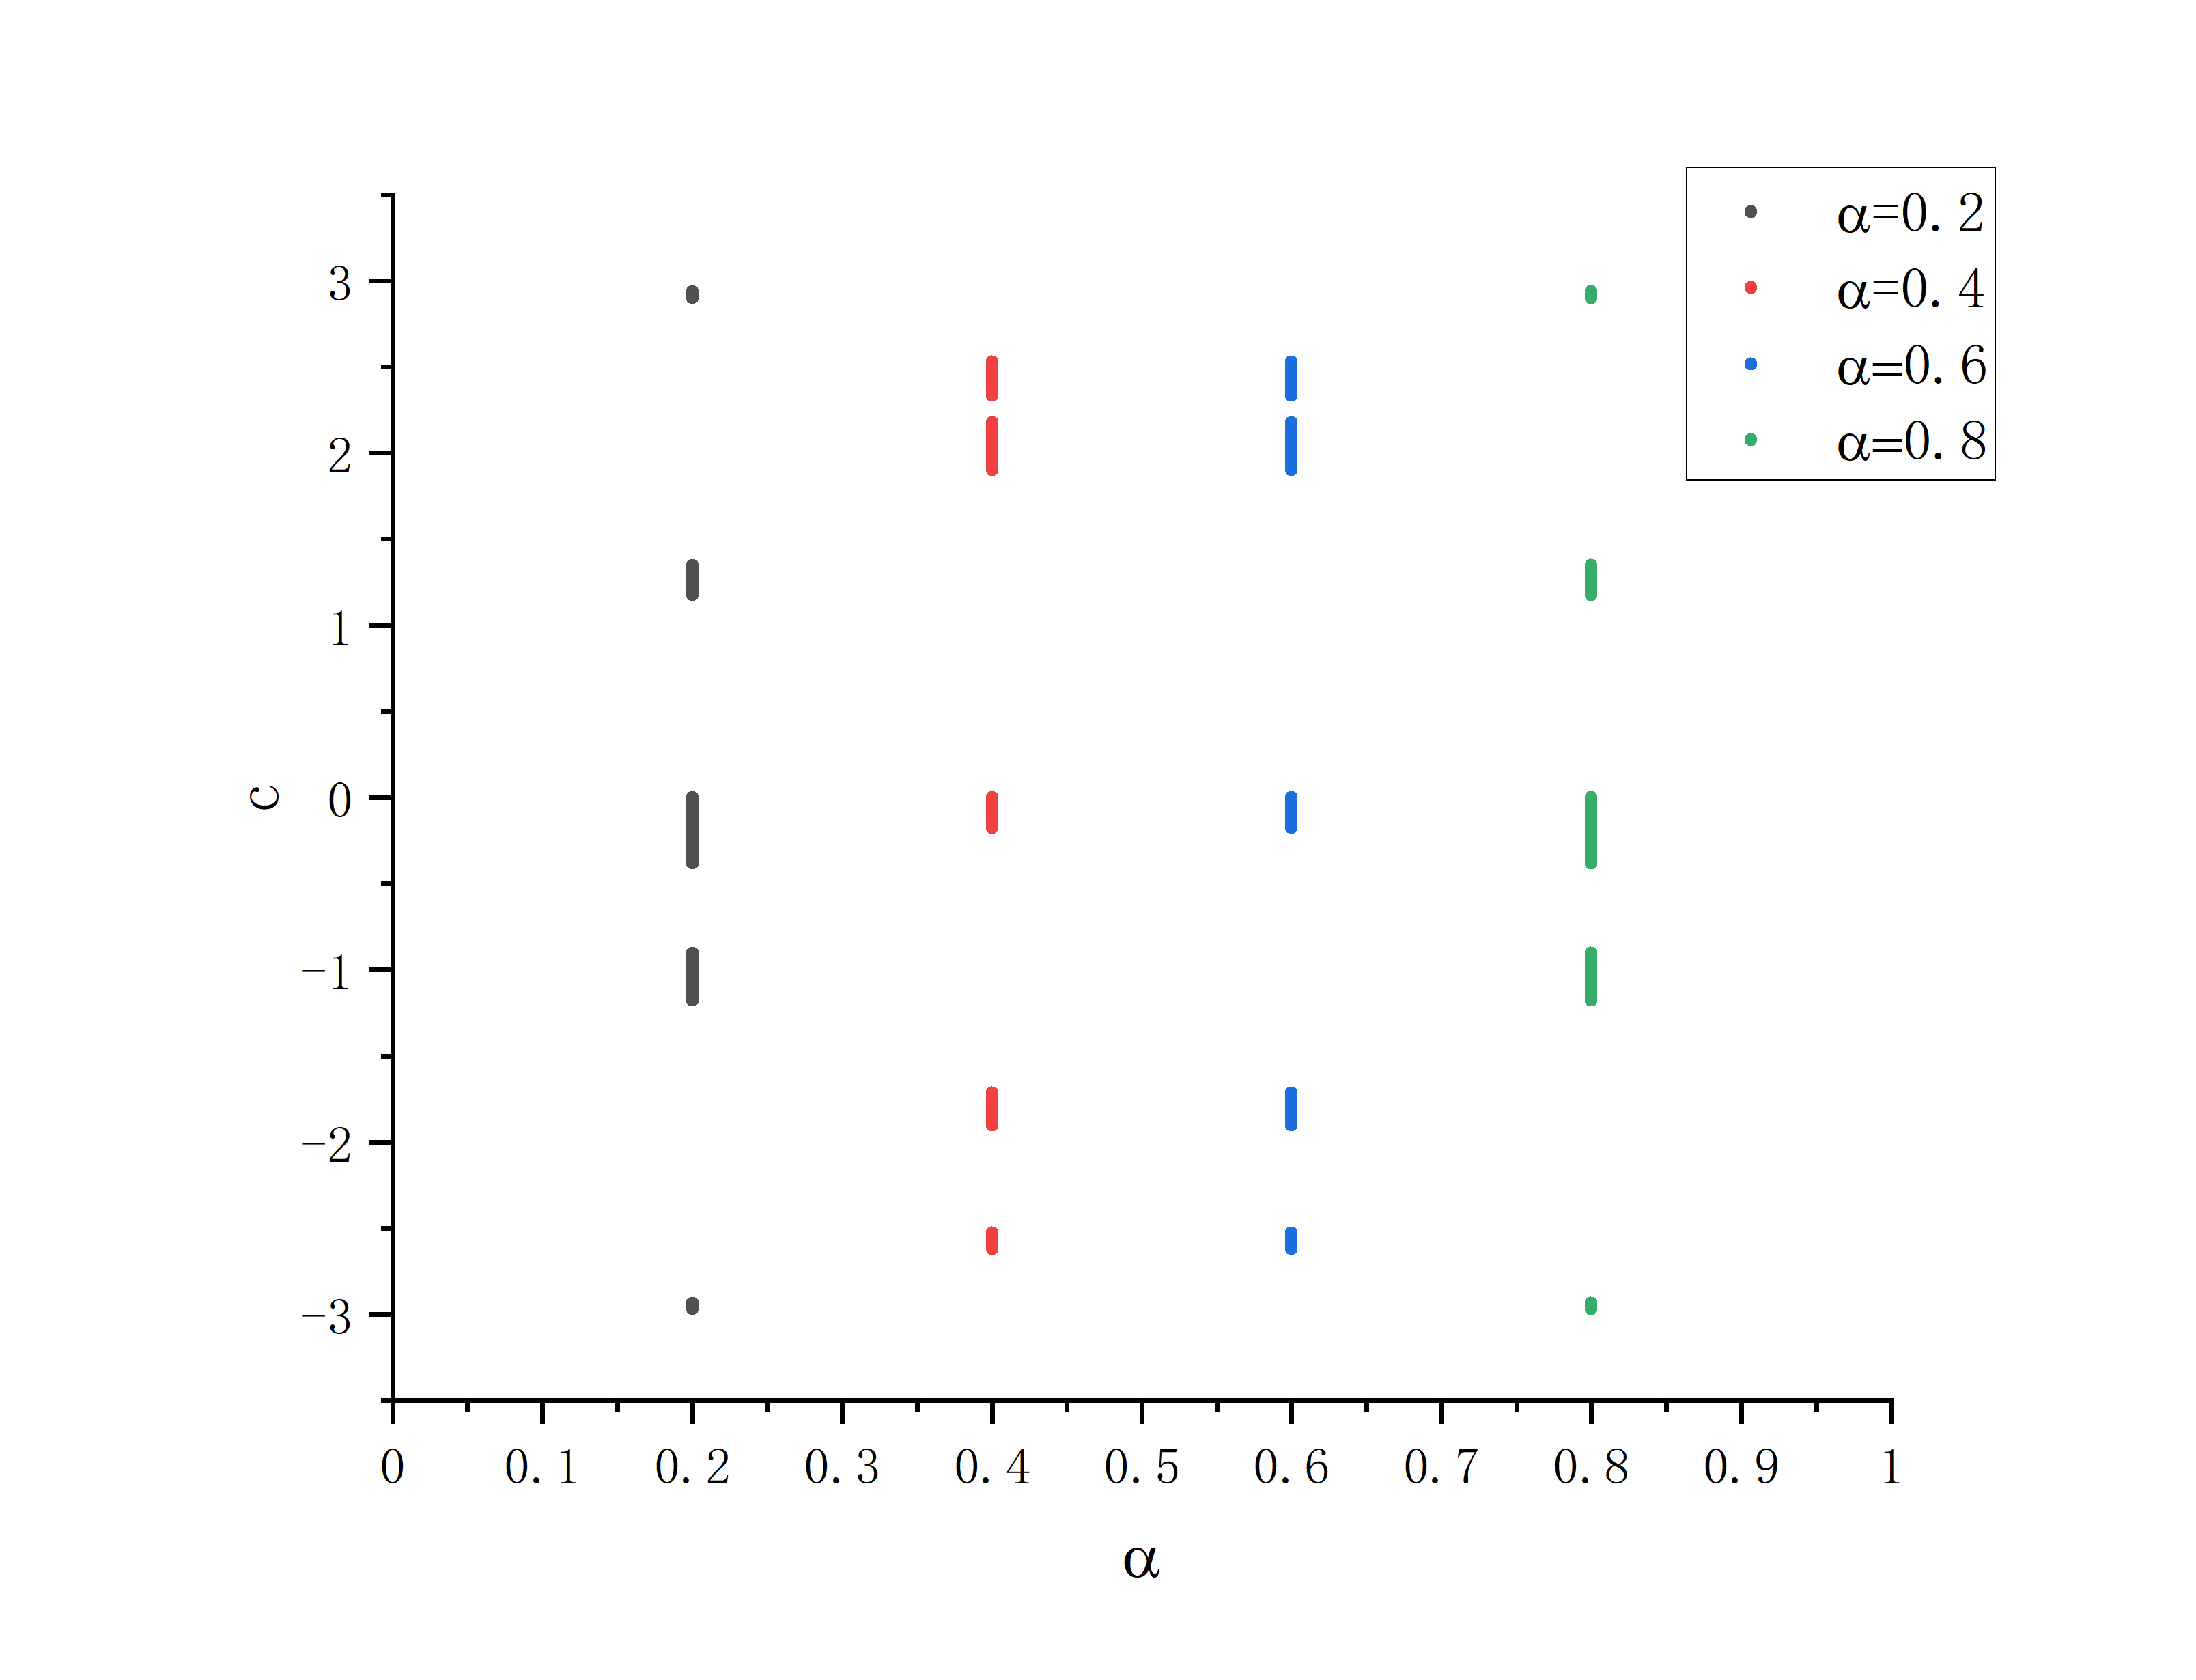
\includegraphics[width=0.6\textwidth]{q5验证特征值劈裂份数与a分子无关.jpg}
        \caption{q5验证特征值劈裂份数与a分子无关}\label{fig:q5验证特征值劈裂份数与a分子无关}
    \end{figure}

    可见,不同的$\alpha$值虽然特征值取值有变化,但是劈裂成的区间数都是一样的。

    \subsection{第六问}

    可以对第四问的代码稍加修改,每取一个$\alpha$,计算一组特征值并输出,具体代码实现见附录。

    这里取

    \[N=720,\gamma=2,\alpha=0.001,0.002,\cdots,0.999\]

    得到数据见"q6.txt"。

    绘制$c-\alpha$图得到Hofstadter蝴蝶。

    \begin{figure}[H]
        \centering
        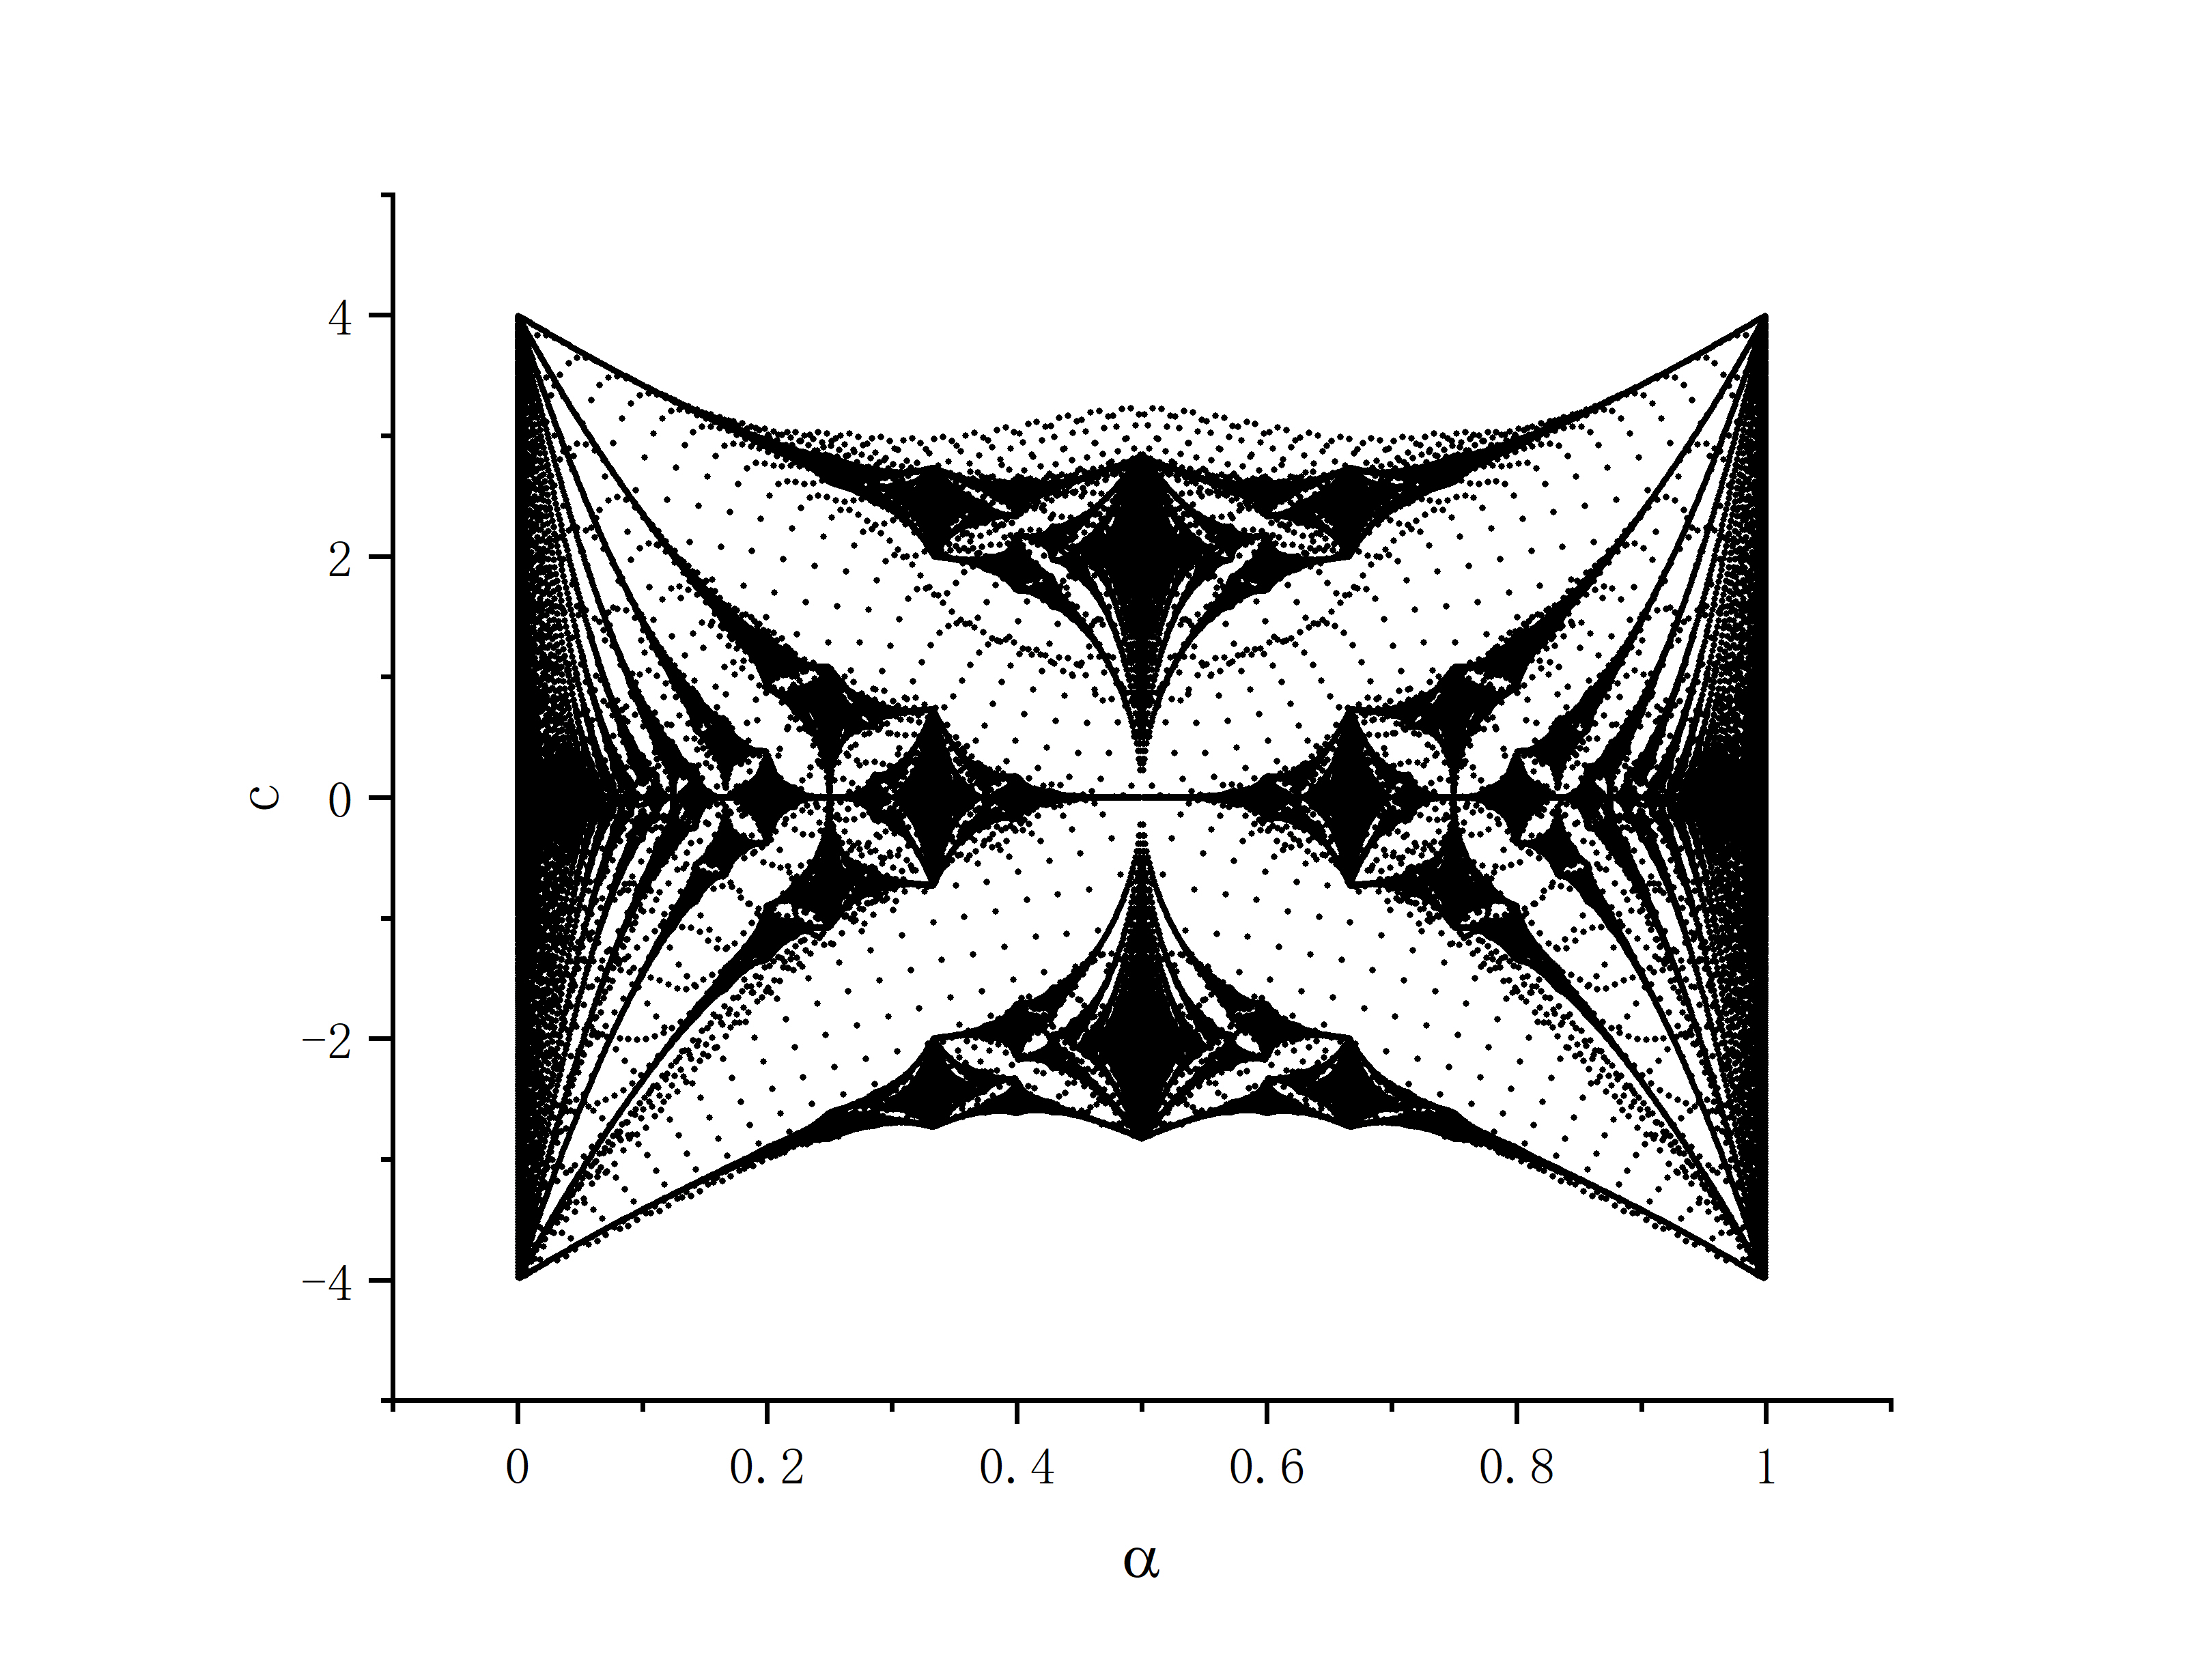
\includegraphics[width=0.6\textwidth]{Hofstadter蝴蝶.jpg}
        \caption{Hofstadter蝴蝶}\label{fig:Hofstadter蝴蝶}
    \end{figure}

    \newpage
    \section{附录}
    \subsection{“matrix.h”头文件}
    \begin{lstlisting}[language=C]
#ifndef __MATRIX_H__
#define __MATRIX_H__

#include<stdio.h>
#include<stdlib.h>
#include<math.h>

#ifndef EPS
#define EPS 1e-7
#endif

#ifndef TOL
#define TOL 1e-10
#endif

#ifndef PI
#define PI 3.1415926535897932
#endif

typedef struct SqMatrix{
    int n;
    double** el;
}SqMatrix;

int sgn(double x){//符号函数
    if(x>=0)return 1;
    return -1;
}
void printMatrix(SqMatrix* A){
    int i,j;
    for ( i = 0; i < A->n; i++)
    {
        for ( j = 0; j < A->n; j++)
        {
            printf("%lf",A->el[i][j]);
            if(j!=A->n-1)printf("\t");
            else printf("\n");
        }
    }
}
double** createNew2DArray(int m,int n){
    int i,j;
    double **a=(double **)malloc(m*sizeof(double *));
    for ( i = 0; i < m; i++)
    {
        a[i]=(double *)malloc(n*sizeof(double));
    }
    for ( i = 0; i < m; i++)
    {
        for ( j = 0; j < n; j++)
        {
            a[i][j]=0;
        }
    }
    return a;
}
SqMatrix* createZeroSqMatrix(int n){
    SqMatrix* p=(SqMatrix*)malloc(sizeof(SqMatrix));
    p->n=n;
    p->el=createNew2DArray(n,n);
    return p;
}
int is_sym_sq(SqMatrix* A){//判断方阵是否对称
    if(A->el==NULL)return 1;
    int i,j;
    for ( i = 0; i < A->n; i++)
    {
        for ( j = i+1; j < A->n; j++)
        {
            if(A->el[i][j]!=A->el[j][i])return 0;
        }
    }
    return 1;
}

double* eigenvalue_sym_sq(SqMatrix* A){//求出实对称方阵的特征值组
    if(!is_sym_sq(A)||A->n<=0)return NULL;
    //Householder变换化为三对角阵
    double *al=(double *)malloc((A->n+1)*sizeof(double));
    double *b=(double *)malloc((A->n+1)*sizeof(double));
    double *au=(double *)malloc((A->n+1)*sizeof(double));
    double *d=(double *)malloc(A->n*sizeof(double));
    if(A->n==1){
        b[1]=A->el[0][0];return b;
    }
    if(A->n==2){
        double b1=A->el[0][0],b2=A->el[1][1],a=A->el[0][1];
        b[1]=(b1+b2+sqrt(pow((b1-b2),2)+4*a*a))/2;
        b[2]=(b1+b2-sqrt(pow((b1-b2),2)+4*a*a))/2;
        return b;
    }
    int i,j,k;
    //printf("entered Householder\n");
    for ( i = 0; i < A->n-2; i++)
    {
        for ( j = i+2; j < A->n; j++)
        {
            if(fabs(A->el[j][i])>EPS) {
                //printf("A(%d,%d)=%.15lf   ",j,i,A->el[j][i]);
                goto Householder;
            }
        }
        continue;

        Householder:
        {
        //printf("start a householder transformation : %d\n",i);
        double sigma=0,beta,uAu;
        for ( j = i+1; j < A->n; j++)
        {
            sigma+=A->el[j][i]*A->el[j][i];
        }
        sigma=sqrt(sigma);
        sigma*=sgn(A->el[i+1][i]);    
        beta=sigma*(sigma+A->el[i+1][i]);
        A->el[i+1][i]+=sigma;//更新u
        //计算Au,储存在uT中
        for ( j = 1; j < A->n-i; j++)
        {
            A->el[i][i+j]=0;
            for ( k = 1; k < A->n-i; k++)
            {
                A->el[i][i+j]+=A->el[i+j][i+k]*A->el[i+k][i];
            }
        }
        //计算uTAu
        uAu=0;
        for ( j = 1; j < A->n-i; j++)
        {
            uAu+=A->el[i+j][i]*A->el[i][i+j];
        }
        //更新A
        for ( j = 1; j < A->n-i; j++)
        {
            for ( k = 1; k < A->n-i; k++)
            {
                A->el[i+j][i+k]-=1/beta*(A->el[i+j][i]*A->el[i][i+k]+A->el[i][i+j]*A->el[i+k][i]);
                A->el[i+j][i+k]+=uAu/(beta*beta)*A->el[i+j][i]*A->el[i+k][i];
            }
        }
        A->el[i+1][i]=A->el[i][i+1]=-sigma;
        for ( j = 2; j < A->n-i; j++)
        {
            A->el[i+j][i]=A->el[i][i+j]=0;
        }
        //printf("%.20lf %.20lf\n",sigma,beta);     
        }
    }
    b[1]=A->el[0][0];
    for ( i = 2; i <= A->n; i++)
    {
        al[i]=A->el[i-1][i-2];
        b[i]=A->el[i-1][i-1];
        au[i-1]=A->el[i-2][i-1];
    }
    //QR迭代求特征值
    int n=A->n;
    double* cosine=(double *)malloc(n*sizeof(double));
    double* sine=(double *)malloc(n*sizeof(double));
    while(n>=2){
        double s=b[n];
        double temp1,temp2;
        b[1]-=s;
        for ( k = 1; k < n; k++)
        {
            b[k+1]-=s;
            double r=sqrt(b[k]*b[k]+al[k+1]*al[k+1]);
            cosine[k]=b[k]/r;sine[k]=al[k+1]/r;
            //左变换
            b[k]=r;al[k+1]=0;
            temp1=au[k],temp2=b[k+1];
            au[k]=temp1*cosine[k]+temp2*sine[k];
            b[k+1]=-temp1*sine[k]+temp2*cosine[k];
            if(k!=n-1){d[k]=au[k+1]*sine[k];au[k+1]*=cosine[k];}
        }
        for ( k = 1; k < n; k++)
        {
            if(k!=1){
                temp1=au[k-1];temp2=d[k-1];
                au[k-1]=temp1*cosine[k]+temp2*sine[k];
                d[k-1]=-temp1*sine[k]+temp2*cosine[k];
            }
            temp1=b[k];temp2=au[k];
            b[k]=temp1*cosine[k]+temp2*sine[k];
            au[k]=temp1*(-sine[k])+temp2*cosine[k];
            temp1=al[k+1];temp2=b[k+1];
            al[k+1]=temp1*cosine[k]+temp2*sine[k];
            b[k+1]=temp1*(-sine[k])+temp2*cosine[k];
            if(k!=n-1)al[k+2]*=cosine[k];

            b[k]+=s;
        }
        b[n]+=s;
        if(fabs(al[n])<EPS){
            al[n]=0;
            //printf("%d\n",n);
            n--;
        }
    }
    return b;
}

#endif
    \end{lstlisting}
    
    \subsection{第一问源代码}
    \begin{lstlisting}[language=C]
//本程序求解第一问,需要手动设置N的取值
#include "matrix.h"
#define N 1024
int main(){
    FILE *fdata=fopen("C:/C_files/HW3/q1-N=1024.txt","w");
    SqMatrix* A;
    A=createZeroSqMatrix(N);
    //构建矩阵
    A->el[A->n-1][0]--;;A->el[0][A->n-1]--;A->el[0][0]=2;
    int i;
    for ( i = 1; i < A->n; i++)
    {
        A->el[i][i]=2;
        A->el[i-1][i]--;
        A->el[i][i-1]--;
    }
    //求特征值
    double* test=eigenvalue_sym_sq(A);
    if(test==NULL)return 0;
    for ( i = 1; i <= A->n; i++)
    {
        fprintf(fdata,"%lf %lf\n",test[i],2*(1-cos(2*PI*i/N)));
    }
    
    return 0;
}
    \end{lstlisting}

    \subsection{第二、三问源代码}
    
    \begin{lstlisting}[language=C]
//本程序求解第二问,并同时完成第三问中解析与数值的比对验算
#include "matrix.h"
double a=1./2;
double r=2;
int n=720;//n>=2

int main(){
    FILE *fdata=fopen("C:/C_files/HW3/q2-N=720.txt","w");
    SqMatrix* A;
    A=createZeroSqMatrix(n);
    A->el[A->n-1][0]=-1;A->el[0][A->n-1]=-1;
    A->el[0][0]=2-r;
    int i;
    for ( i = 1; i < A->n ; i++)
    {
        A->el[i-1][i]=A->el[i][i-1]=-1;
        A->el[i][i]=2+r*cos(2*PI*(i+1)*a);
    }
    double *test=eigenvalue_sym_sq(A);
    if(test==NULL)return 0;
    for(i=1;i<=A->n;i++){
        fprintf(fdata,"%lf  %lf %lf\n",2-test[i],(2-test[i])*(2-test[i]),r*r+2*(1+cos(4*PI*i/n)));
    }
    return 0;
}
    \end{lstlisting}
    
    \subsection{第四、五问源代码}

    \begin{lstlisting}[language=C]
#include "matrix.h"
\\本程序求解第4,5问;需要手动调置a,r,n;
double a=1./4;
double r=-2;
int n=720;//n>=2

int main(){
    FILE *fdata=fopen("C:/C_files/HW3/q4-explore-r=-2.txt","w");
    SqMatrix* A;
    A=createZeroSqMatrix(n);
    A->el[A->n-1][0]=-1;A->el[0][A->n-1]=-1;
    A->el[0][0]=2+r*cos(2*PI*a);
    int i;
    for ( i = 1; i < A->n ; i++)
    {
        A->el[i-1][i]=A->el[i][i-1]=-1;
        A->el[i][i]=2+r*cos(2*PI*(i+1)*a);
    }
    double *test=eigenvalue_sym_sq(A);
    if(test==NULL)return 0;
    for(i=1;i<=A->n;i++){
        fprintf(fdata,"%lf\n",2-test[i]);
    }
    return 0;
}
    \end{lstlisting}

    \subsection{第六问源代码}
    \begin{lstlisting}[language=C]
#include "matrix.h"
#define ITV 1e-3//a的取值步长
#define N 720
double a=ITV;
double r=2;

int main(){
    FILE *fdata=fopen("C:/C_files/HW3/q6.txt","w");
    for(a=ITV;a<1;a+=ITV)
    {
    SqMatrix* A;
    A=createZeroSqMatrix(N);
    A->el[A->n-1][0]=-1;A->el[0][A->n-1]=-1;
    A->el[0][0]=2+r*cos(2*PI*a);
    int i;
    for ( i = 1; i < A->n ; i++)
    {
        A->el[i-1][i]=A->el[i][i-1]=-1;
        A->el[i][i]=2+r*cos(2*PI*(i+1)*a);
    }
    double *test=eigenvalue_sym_sq(A);
    if(test==NULL)return 0;
    for(i=1;i<=A->n;i++){
        fprintf(fdata,"%lf  %lf\n",a,test[i]);
    }
     printf("a=%lf finished...\n",a);
    }
    fclose(fdata);
    return 0;
}
    \end{lstlisting}
    \begin{thebibliography}{99}  
        \bibitem{ref1}李庆扬,王能超,易大义:数值分析,261-263页,269-271页,2008年12月第五版
    \end{thebibliography}
\end{document}